\documentclass[aspectratio=169]{beamer}
\usetheme{Madrid}
%\usecolortheme{beetle}
%\usecolortheme{rose}

\usepackage{graphicx}
\usepackage[utf8]{inputenc}
\usepackage{hyperref}
\usepackage{listings}

%\setbeamertemplate{footline}[frame number]

\begin{document}

\title{
	%
\includegraphics[width=3cm]{logo_conacyt}\hspace*{4.75cm} %
\includegraphics[width=1.8cm]{cidetec}\hspace*{4.75cm} 
	\\Computer Vision with Deep Learning}  
\subtitle{YOLO detection} 
\author[J.I. Vasquez]{\\Juan Irving Vásquez \\@juan1rving}
\date{\today \copyright}
\institute{jivg.org}
%\institute{Centro de Innovación y Desarrollo Tecnológico en Cómputo}
% logo of my university
%\titlegraphic{
\includegraphics[width=2cm]{logo_conacyt}\hspace*{4.75cm}}
\frame{\titlepage}


\section{Object detection}


\begin{frame}
\frametitle{Object detection}
\begin{itemize}
	\item Object detection vs classification
\end{itemize}
\begin{center}
	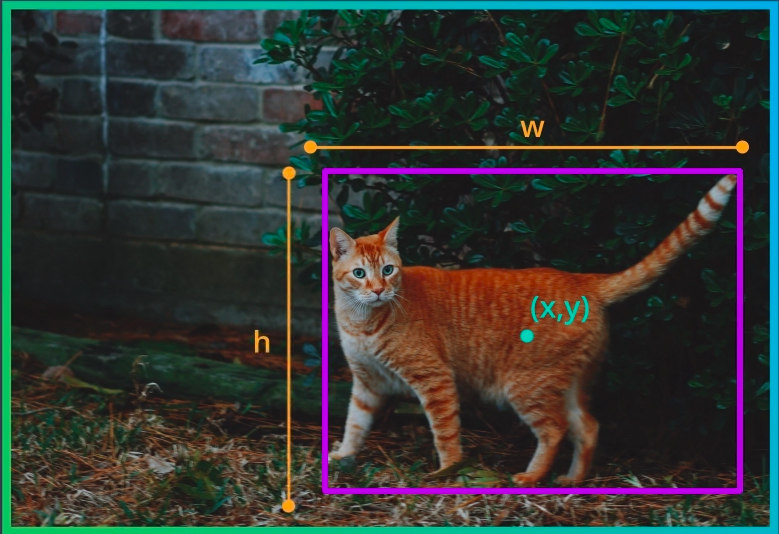
\includegraphics[height=0.6\textheight]{cat}
\end{center}
\end{frame}


{\usebackgroundtemplate{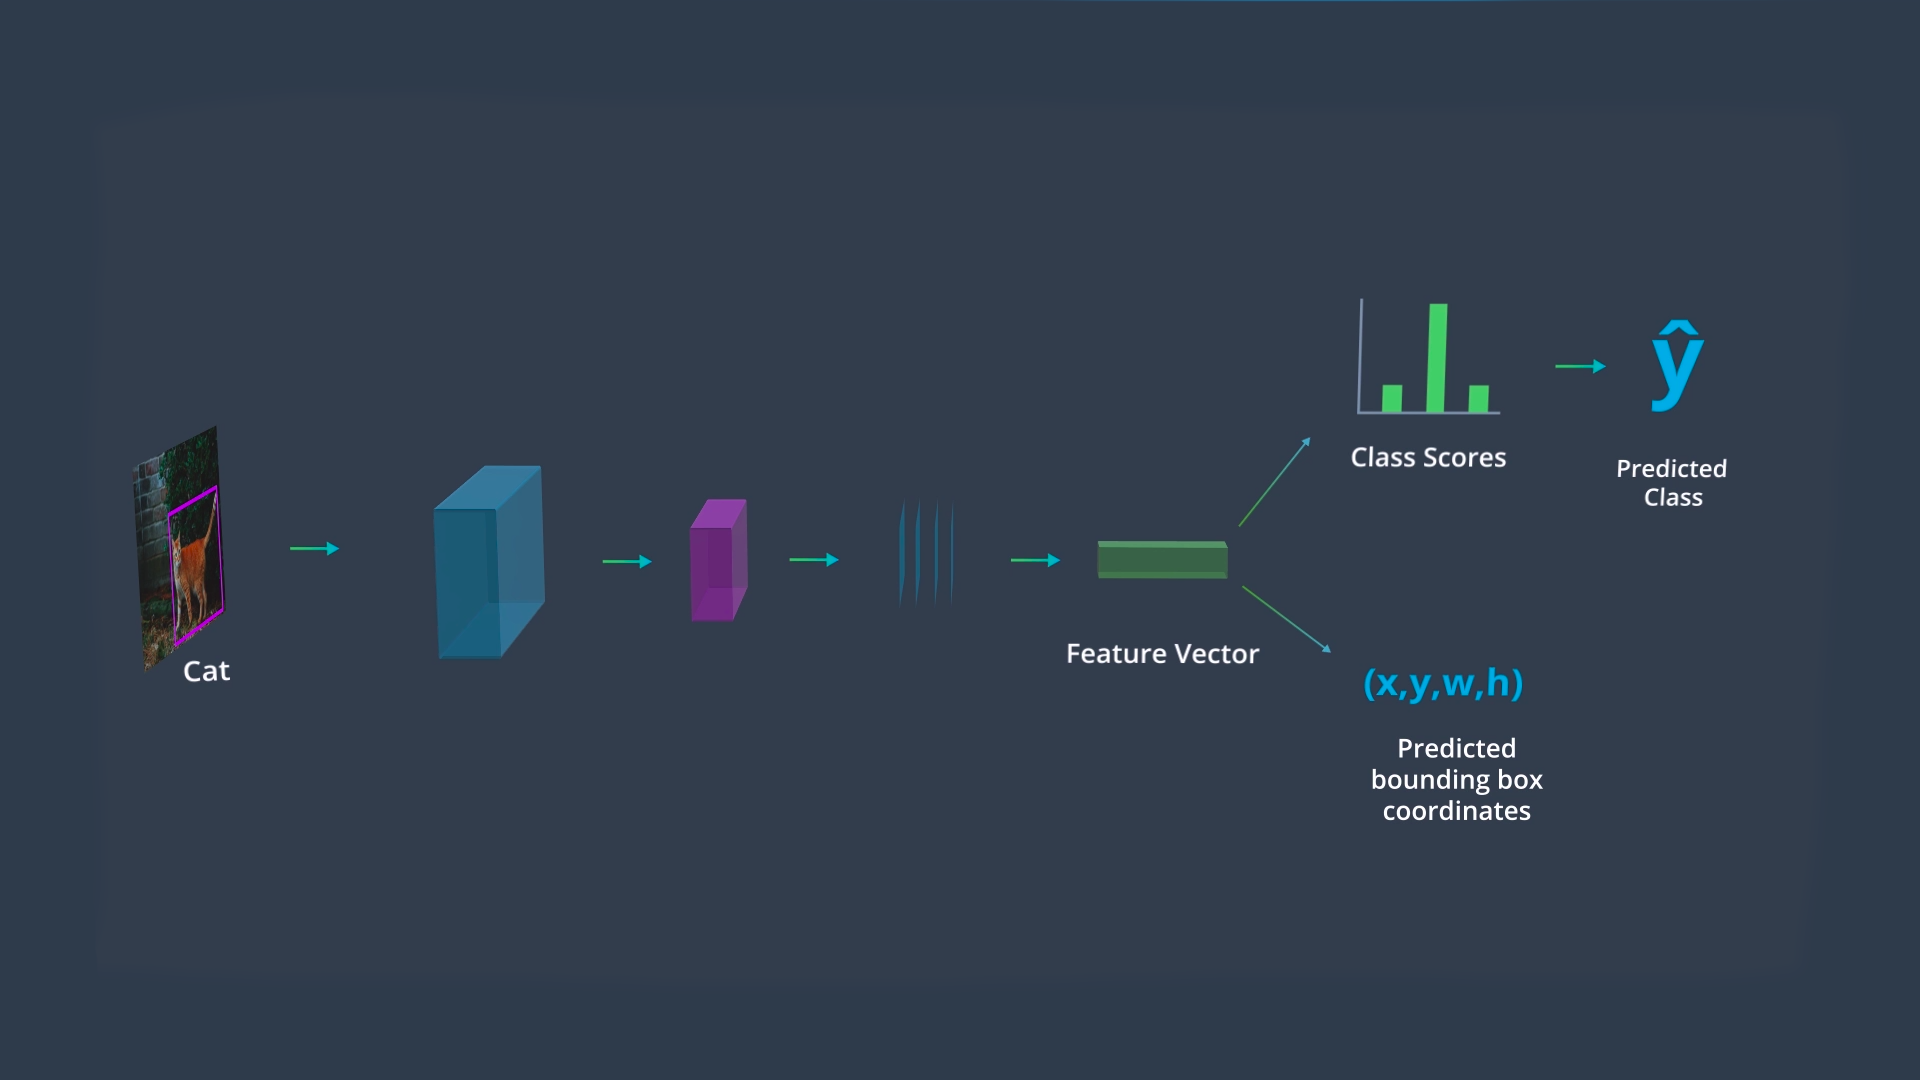
\includegraphics[width=1.0\paperwidth]{position}}%
\begin{frame}
\frametitle{Object detection}
\framesubtitle{Using the same architecture}
\end{frame}
}




\begin{frame}
\frametitle{Multiple objects}
\begin{itemize}
	\item How can we detect multiple objects?
\end{itemize}
\begin{center}
	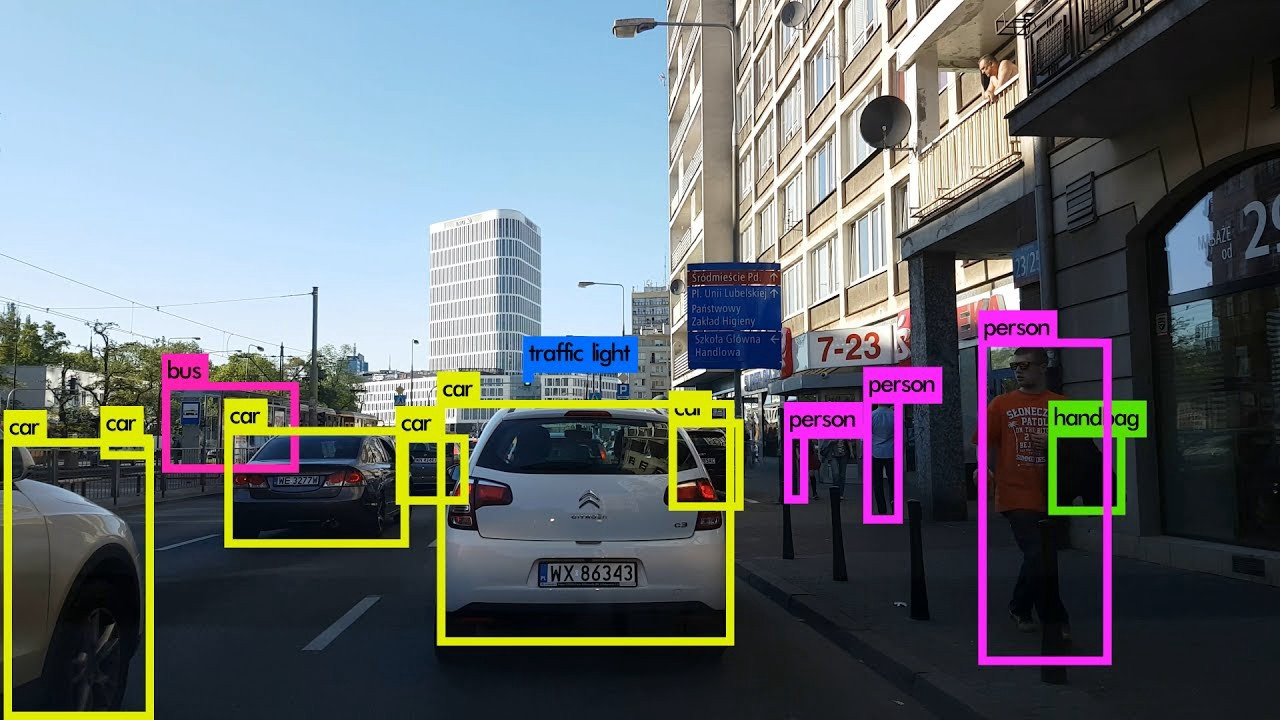
\includegraphics[height=0.6\textheight]{multiple}
\end{center}
\end{frame}


\begin{frame}
\frametitle{Multiple objects}
\begin{itemize}
	\item Sliding window \footnote{Felzenszwalb, Pedro F., et al. "Object detection with discriminatively trained part-based models." IEEE transactions on pattern analysis and machine intelligence 32.9 (2009): 1627-1645.}
	\begin{center}
		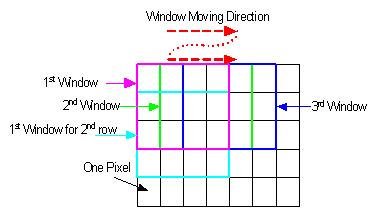
\includegraphics[height=0.5\textheight]{swo}
	\end{center}
	\item Extremely expensive
\end{itemize}
\end{frame}


\begin{frame}
\frametitle{Region proposals}
\begin{itemize}
	\item Regions only for areas which might contain an object. \footnote{Girshick, Ross, et al. "Rich feature hierarchies for accurate object detection and semantic segmentation." Proceedings of the IEEE conference on computer vision and pattern recognition. 2014.}
	\item We may use boundaries, regions, texture, feature points... etc.
\end{itemize}
\begin{center}
	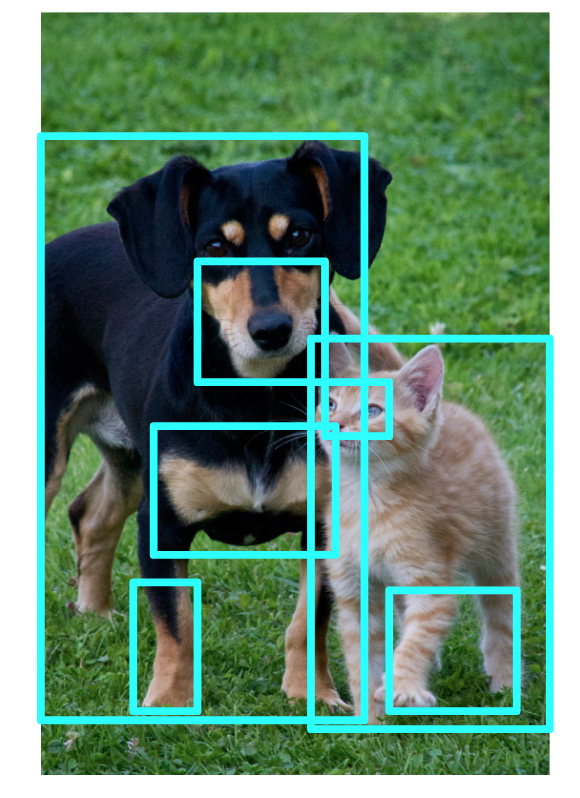
\includegraphics[height=0.6\textheight]{rp}
\end{center}
\end{frame}


{\usebackgroundtemplate{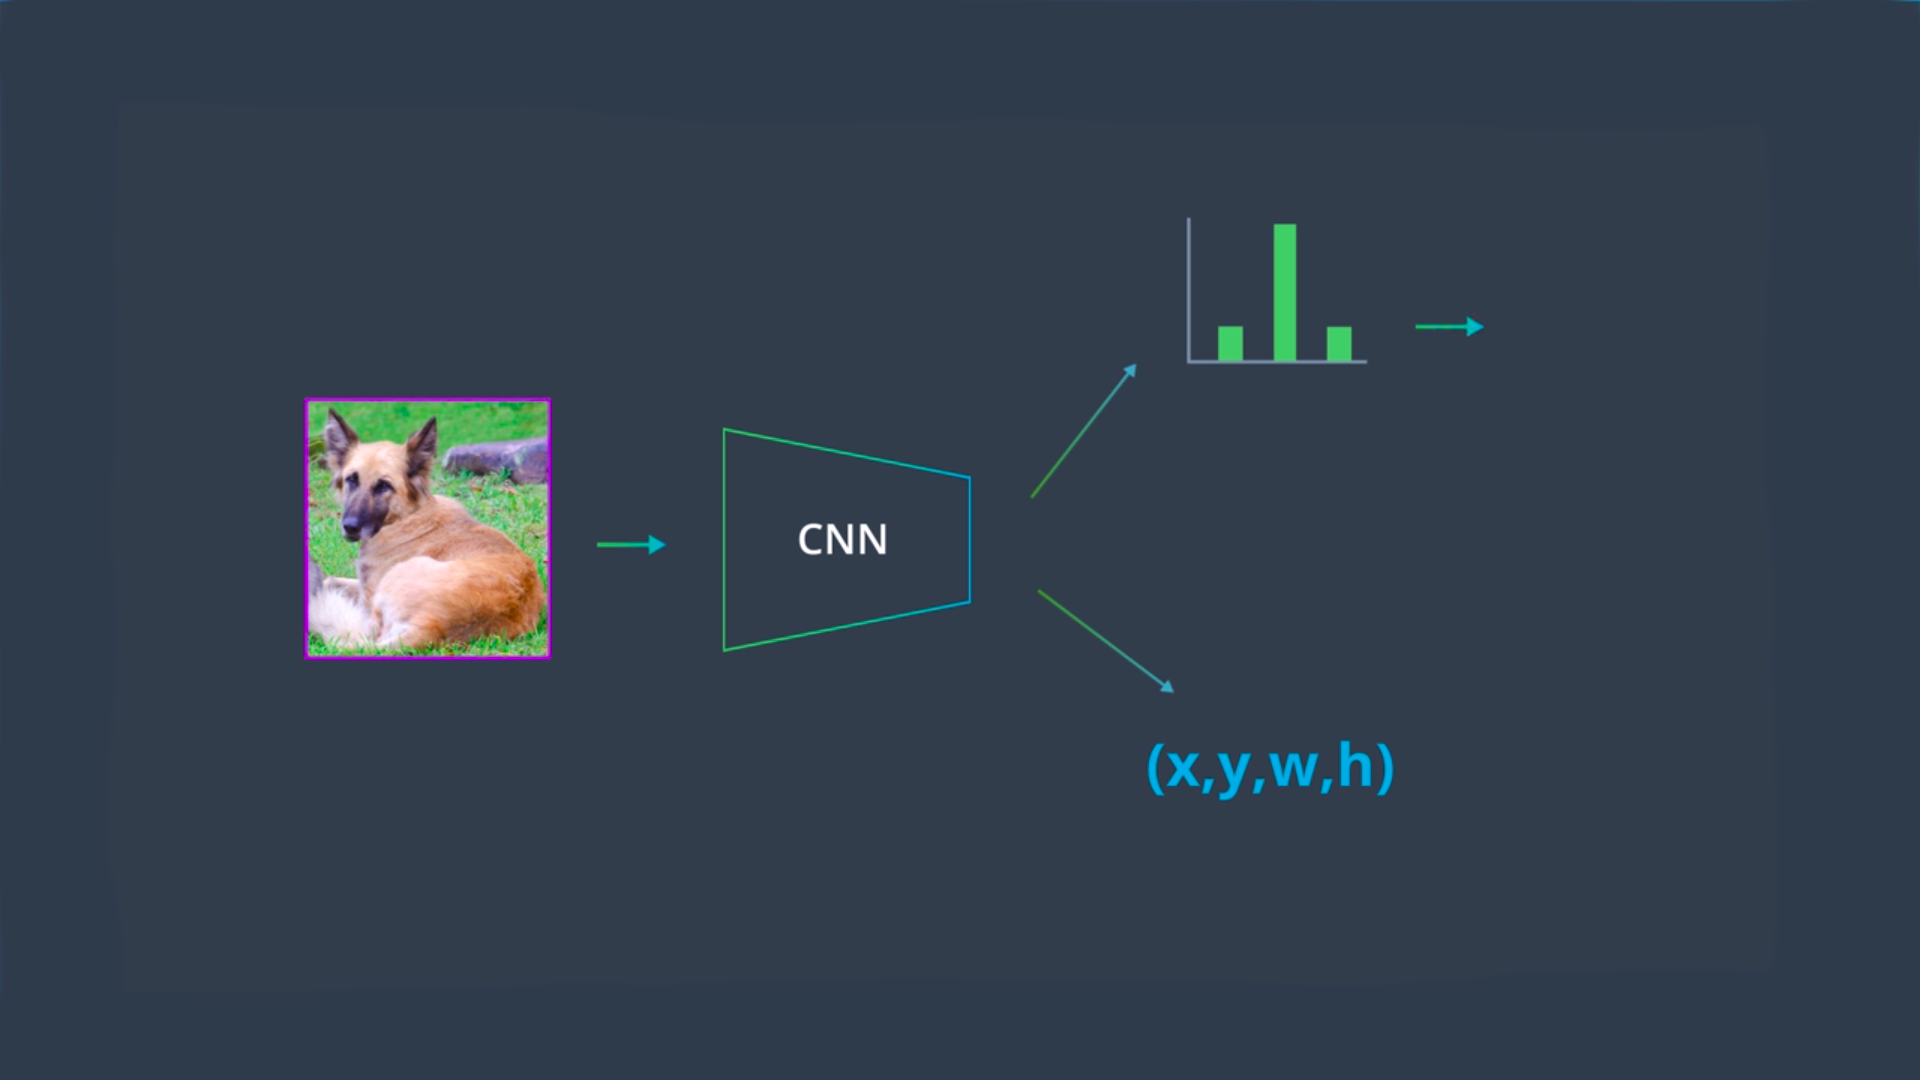
\includegraphics[width=1.0\paperwidth]{rcnn}}%
\begin{frame}
\frametitle{R-CNN}
\subtitle{Region convolutional neural networks}
\vspace{6cm}
\begin{itemize}
	\item \textcolor{white}{input: proposed region; output: label or background}
\end{itemize}
%\begin{center}
%	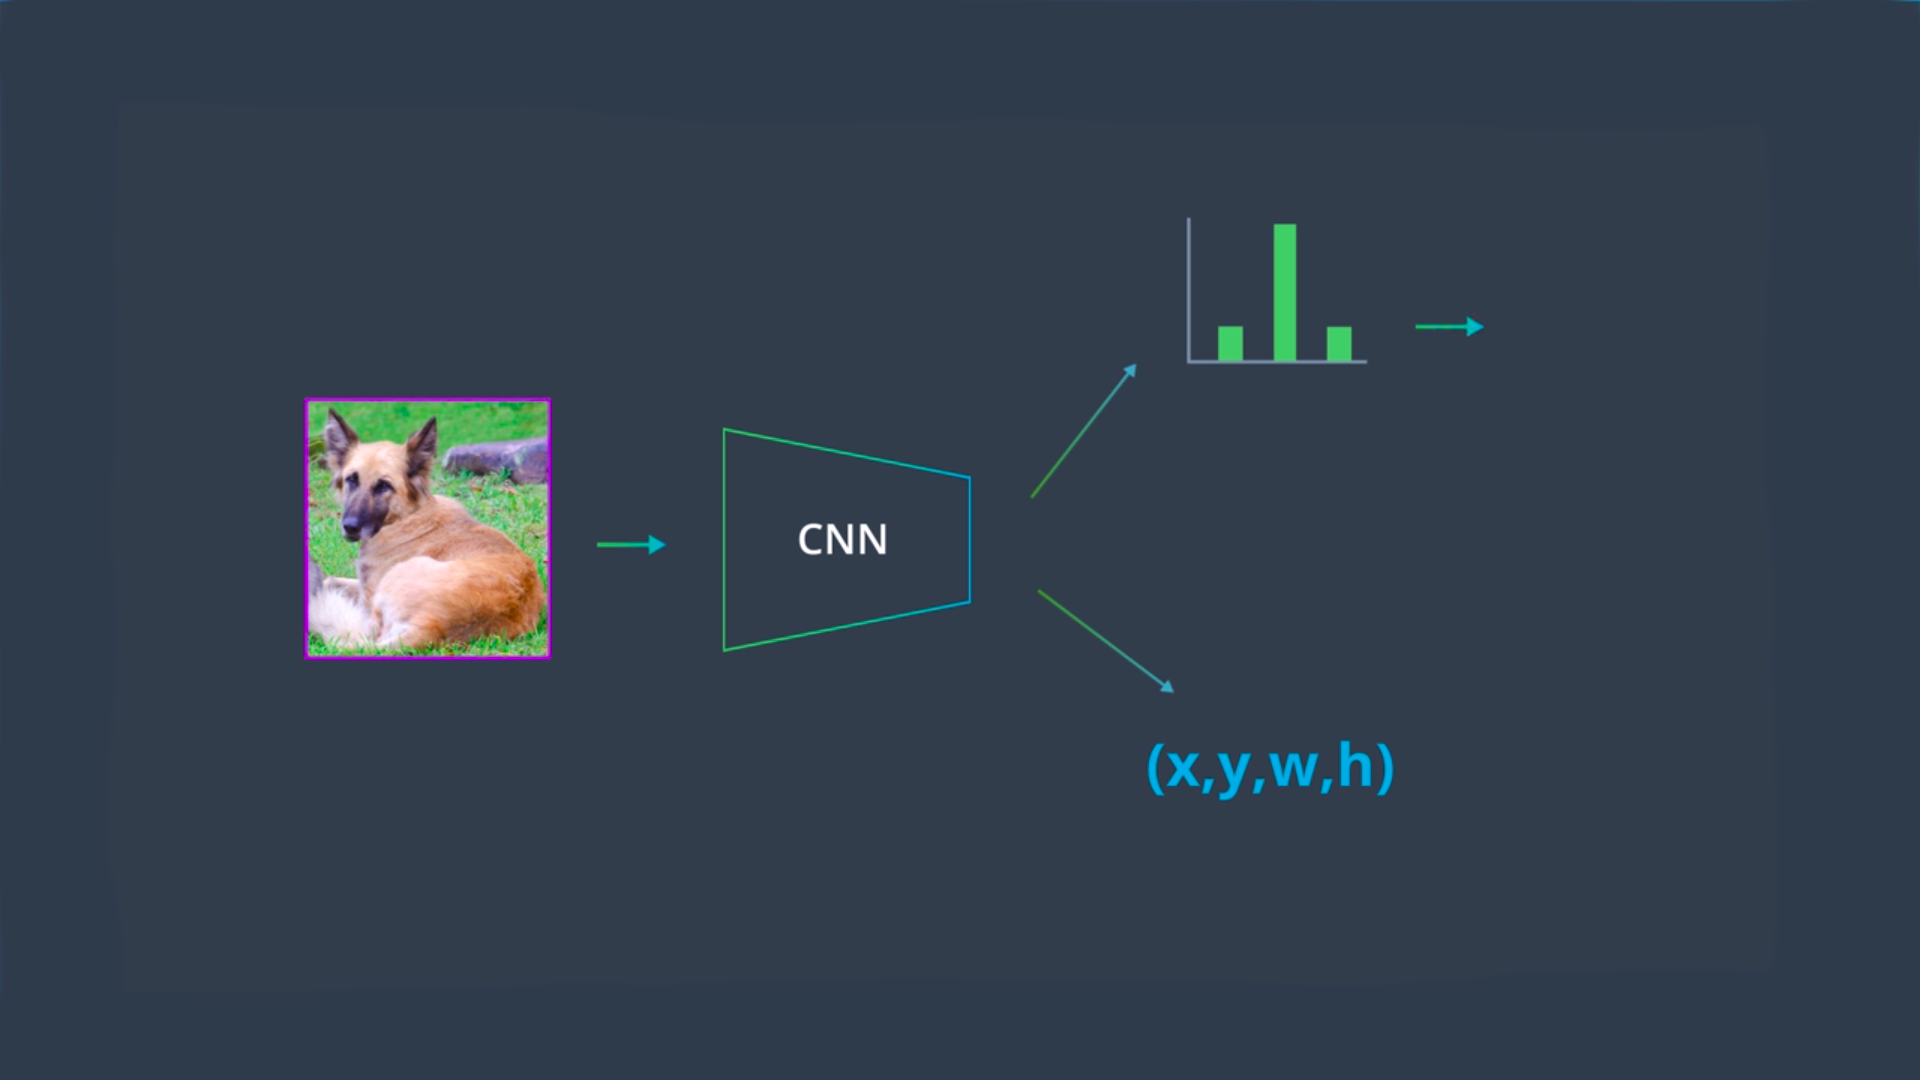
\includegraphics[width=\linewidth]{rcnn}
%\end{center}
\end{frame}
}

\section{YOLO}


\begin{frame}
\frametitle{YOLO}
\framesubtitle{You only look once \footnote{Redmon, Joseph, et al. "You only look once: Unified, real-time object detection." Proceedings of the IEEE conference on computer vision and pattern recognition. 2016.}}
%\begin{itemize}
%	\item You only look once
%	\item 
%\end{itemize}
\begin{center}
	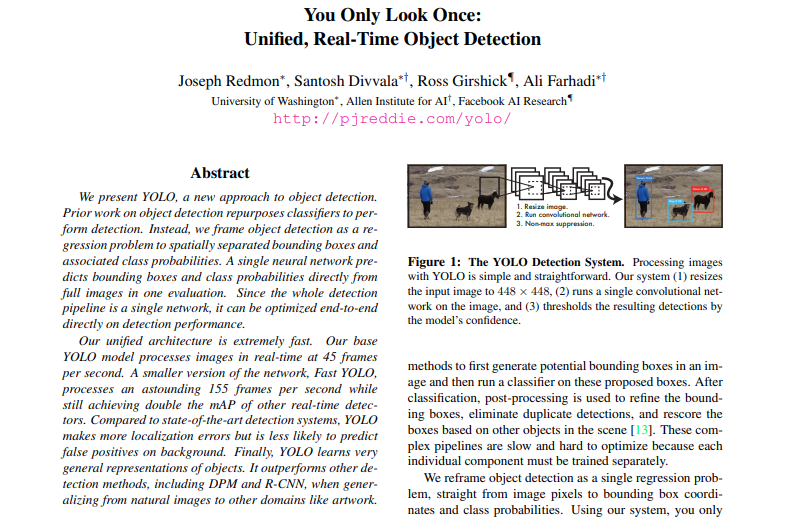
\includegraphics[height=0.7\textheight]{yolo}
\end{center}
\end{frame}


{\usebackgroundtemplate{
\includegraphics[width=1.0\paperwidth]{background}}%
\begin{frame}
\frametitle{YOLO preliminaries}
\framesubtitle{Output}
\begin{itemize}
	\item \textcolor{white}{The output should be a vector}
\end{itemize}
\begin{center}
		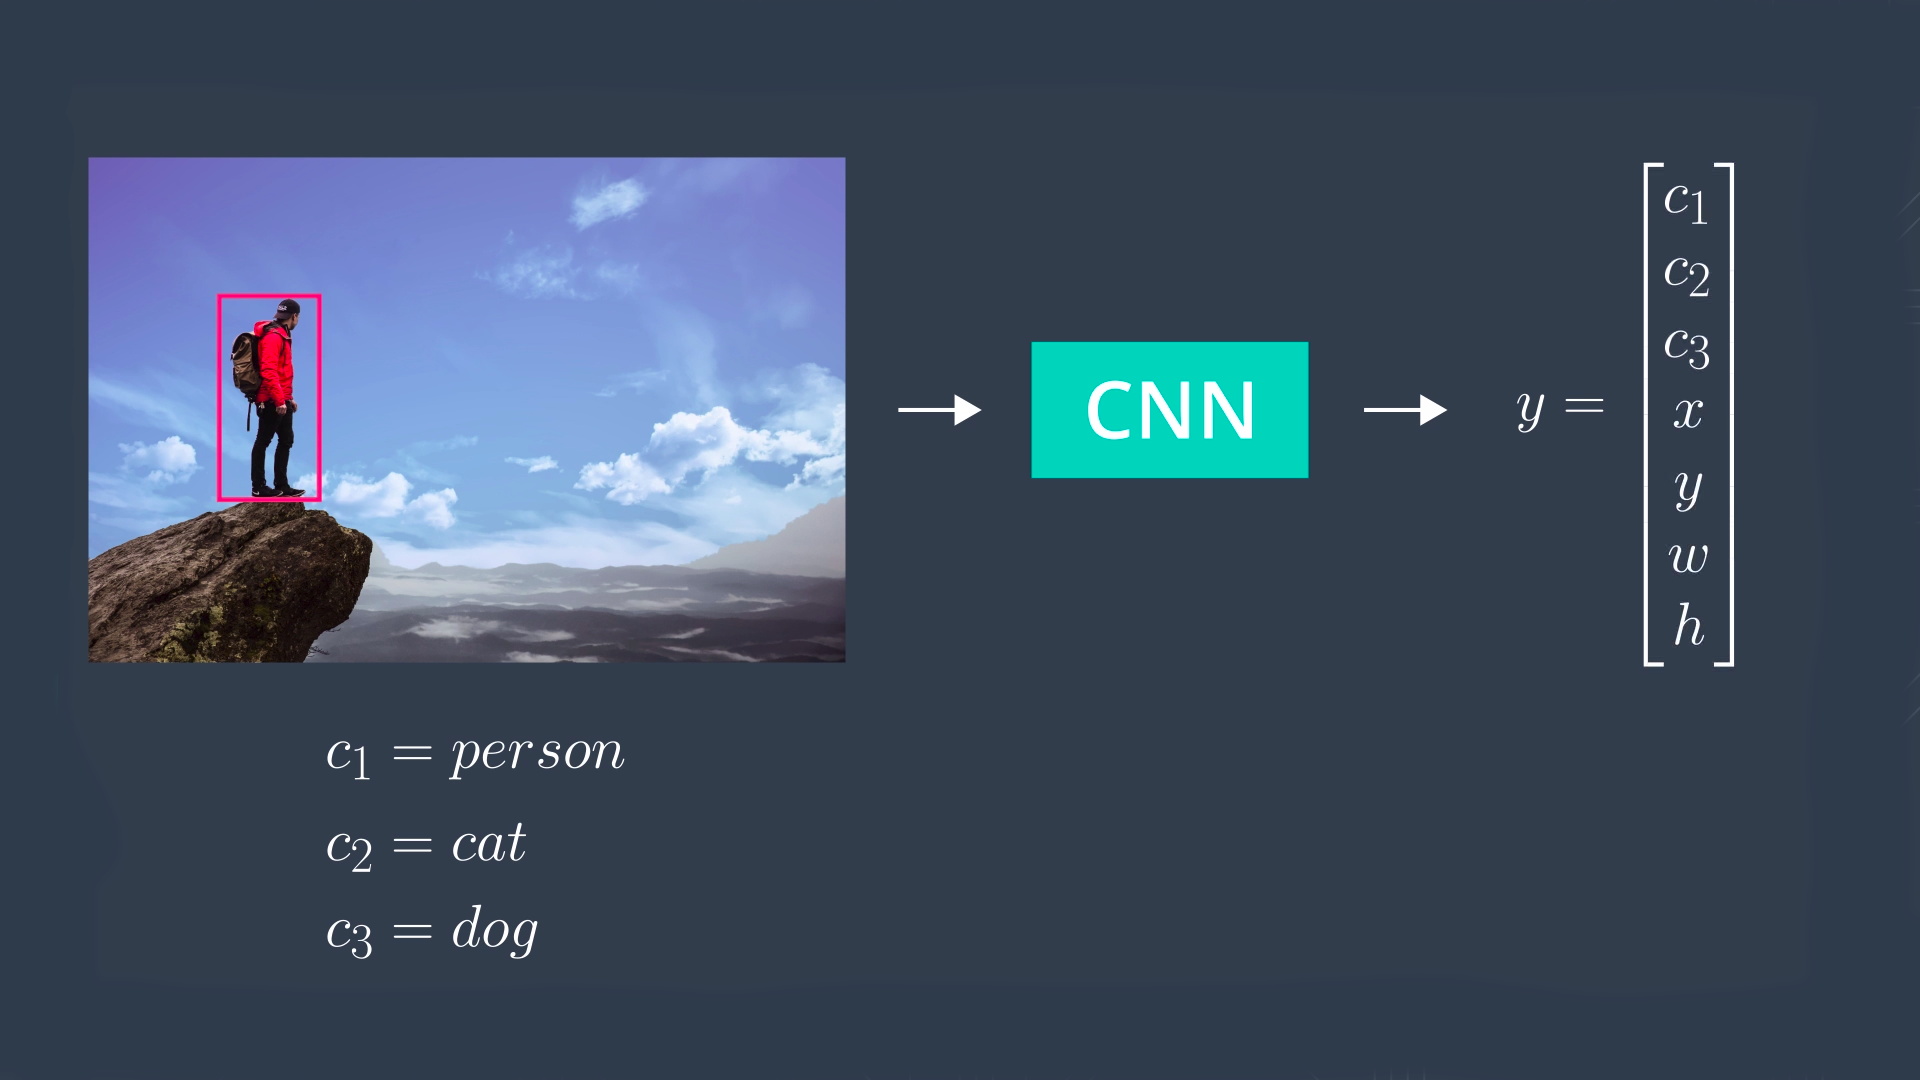
\includegraphics[height=0.7\textheight]{yoloout}
\end{center}
\end{frame}
}


{\usebackgroundtemplate{
\includegraphics[width=1.0\paperwidth]{background}}%
\begin{frame}
\frametitle{Sliding window}
%\frametitle{YOLO preliminaries}
\begin{itemize}
	\item \textcolor{white}{$p_c$ outputs the probability that an object is in the window.}
	\item \textcolor{white}{It works great but it is expensive.}
\end{itemize}
\begin{center}
	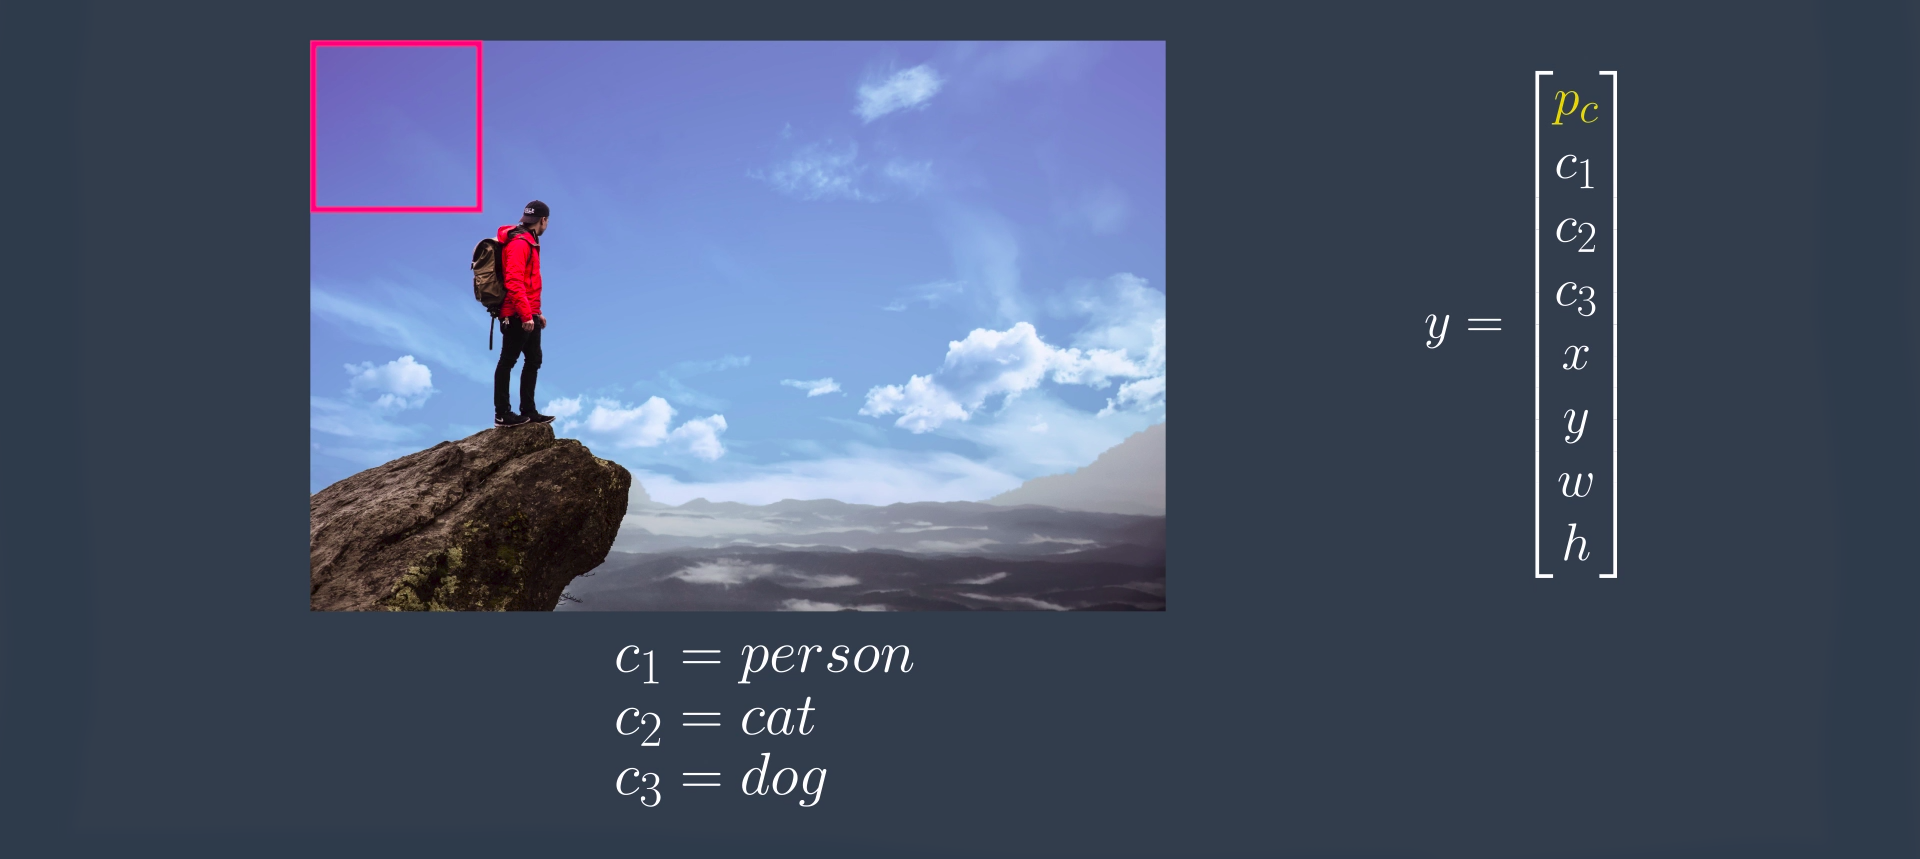
\includegraphics[height=0.7\textheight]{swyolo}
\end{center}
\end{frame}
}


\begin{frame}
\frametitle{Analyzing sliding windows}
\begin{itemize}
	\item Sliding window
\end{itemize}
\begin{center}
	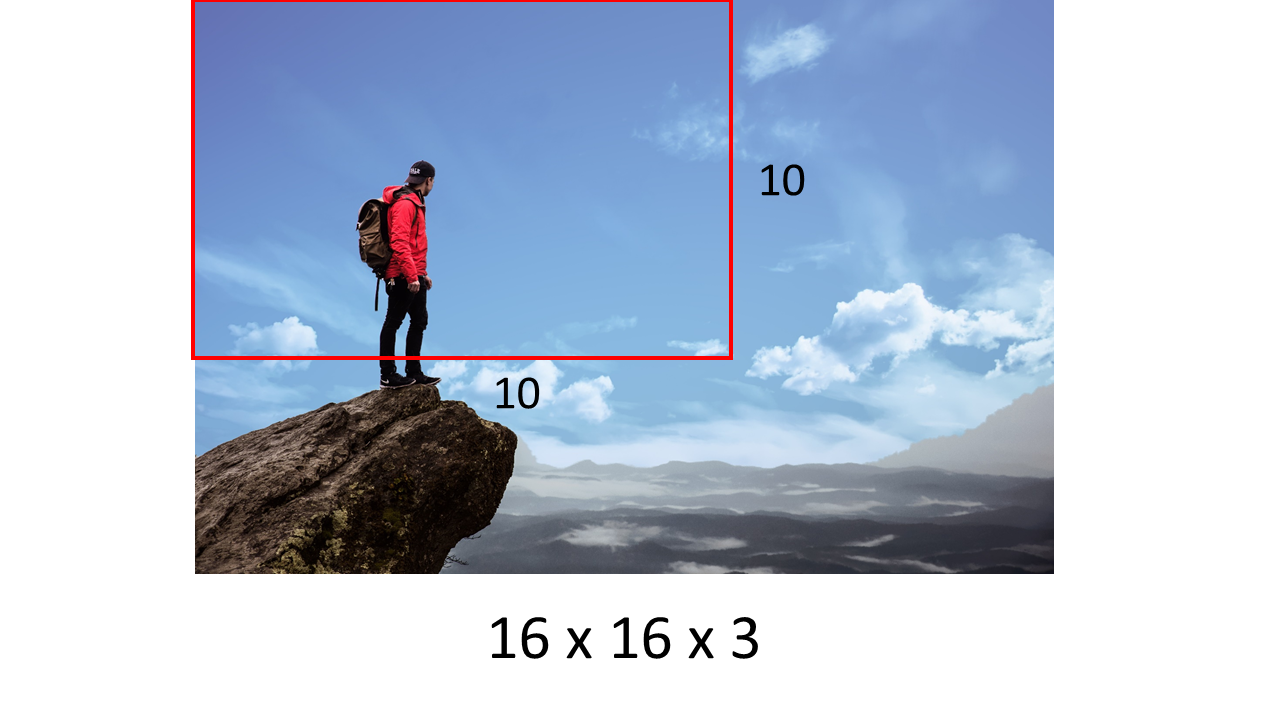
\includegraphics[width=0.45\linewidth]{diapositiva2}
	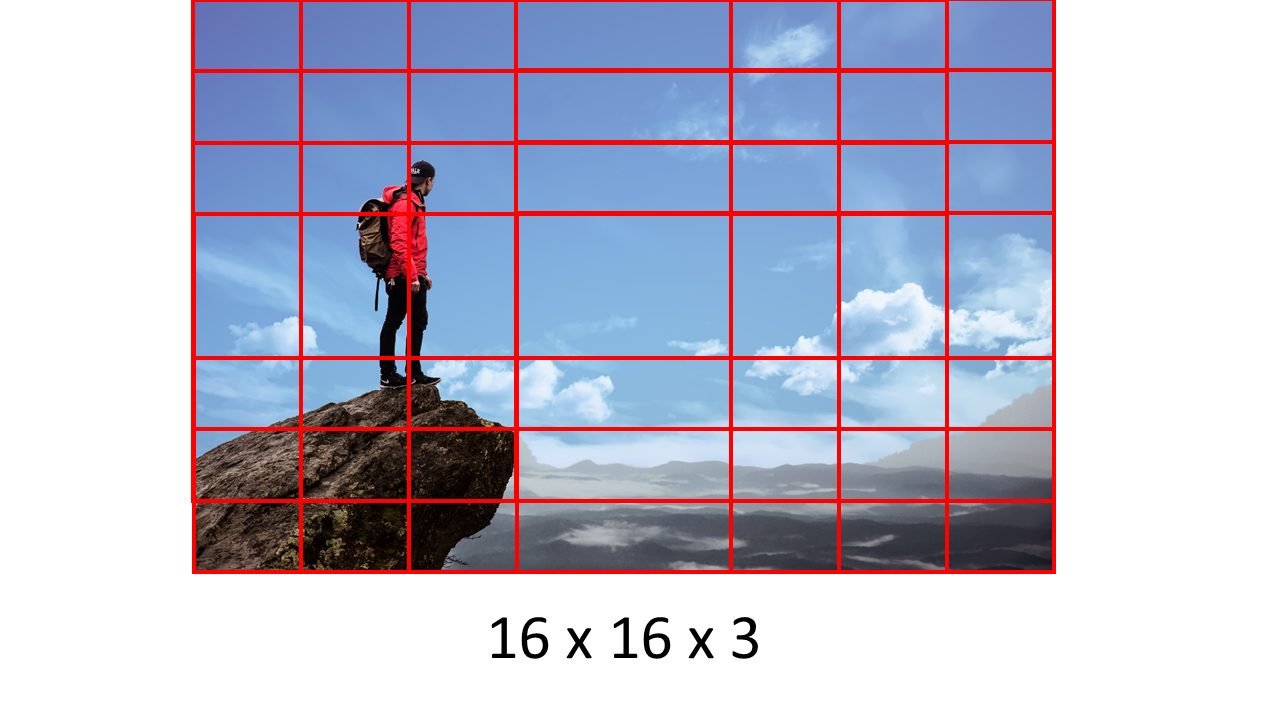
\includegraphics[width=0.45\linewidth]{diapositiva3}
\end{center}
\end{frame}


%\begin{frame}
%\frametitle{Analyzing sliding windows}
%\begin{itemize}
%	\item Sliding window
%\end{itemize}
%\begin{center}
%	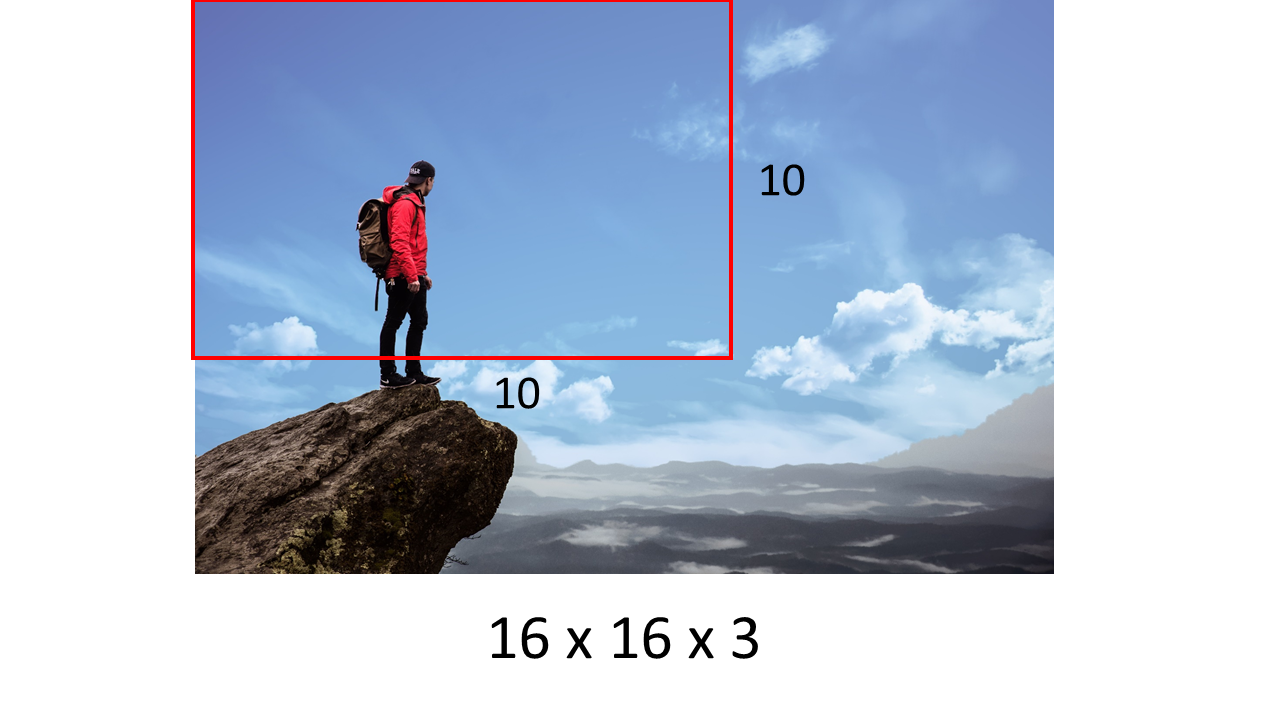
\includegraphics[width=0.45\linewidth]{diapositiva2}
%	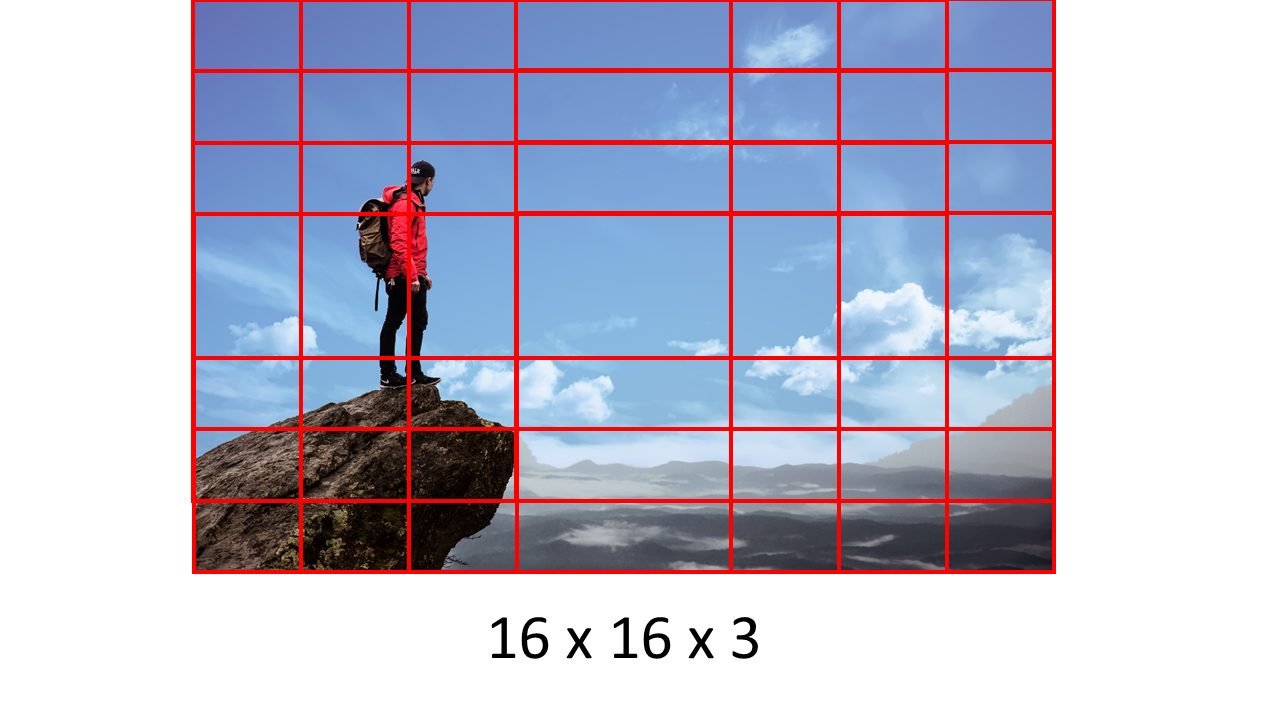
\includegraphics[width=0.45\linewidth]{diapositiva3}
%\end{center}
%\end{frame}


\begin{frame}
\frametitle{Analyzing sliding windows}
\begin{itemize}
	\item Passing the window through a CNN
		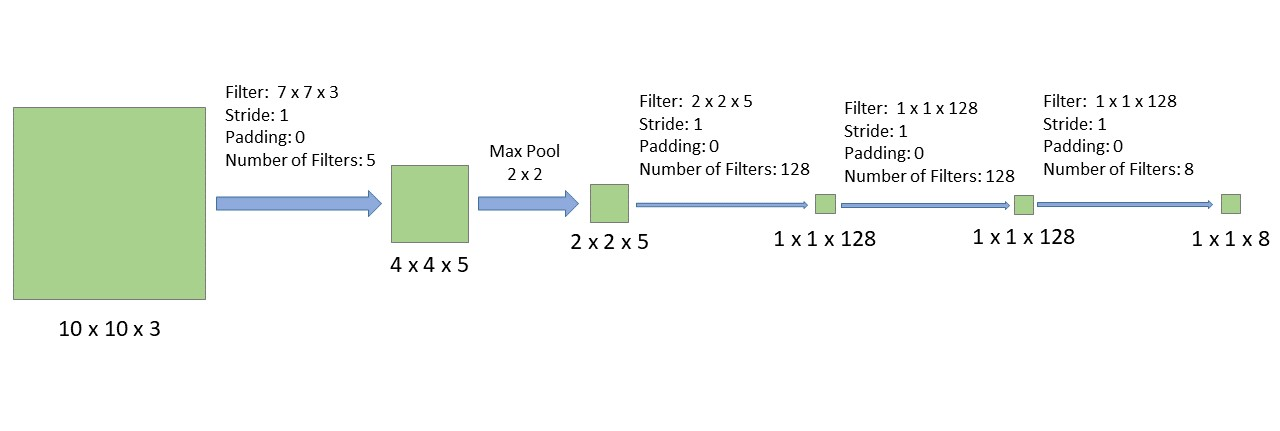
\includegraphics[height=0.4\textheight]{diapositiva4}
	\item Whole image through the CNN
		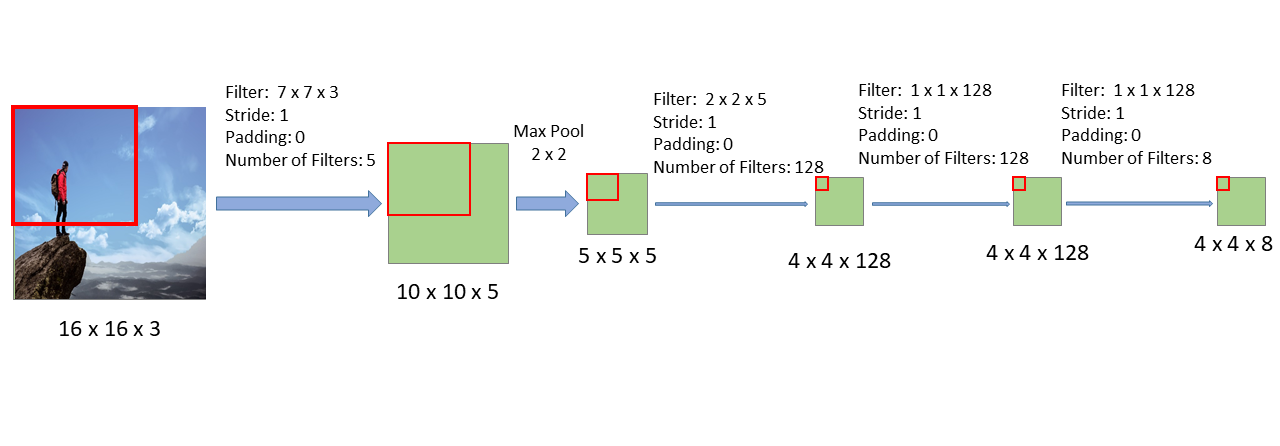
\includegraphics[height=0.4\textheight]{diapositiva5-1}
\end{itemize}
\end{frame}


\begin{frame}
\frametitle{Eureka!}
\begin{itemize}
	\item The windows are represented in the last layer of the CNN!
\end{itemize}
\begin{figure}
	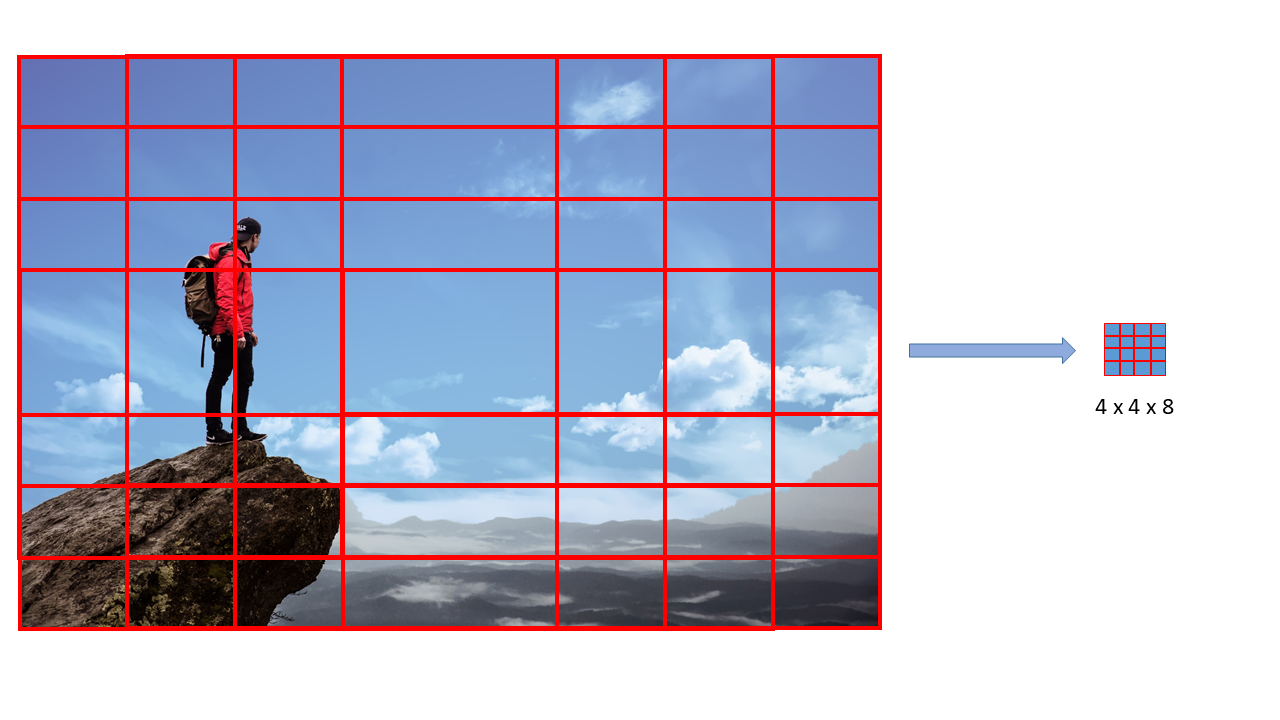
\includegraphics[height=0.7\textheight]{last}
\end{figure}

\end{frame}


{\usebackgroundtemplate{
\includegraphics[width=1.0\paperwidth]{background}}%
\begin{frame}
\frametitle{A grid instead windows}
\framesubtitle{Improving localization with cells}
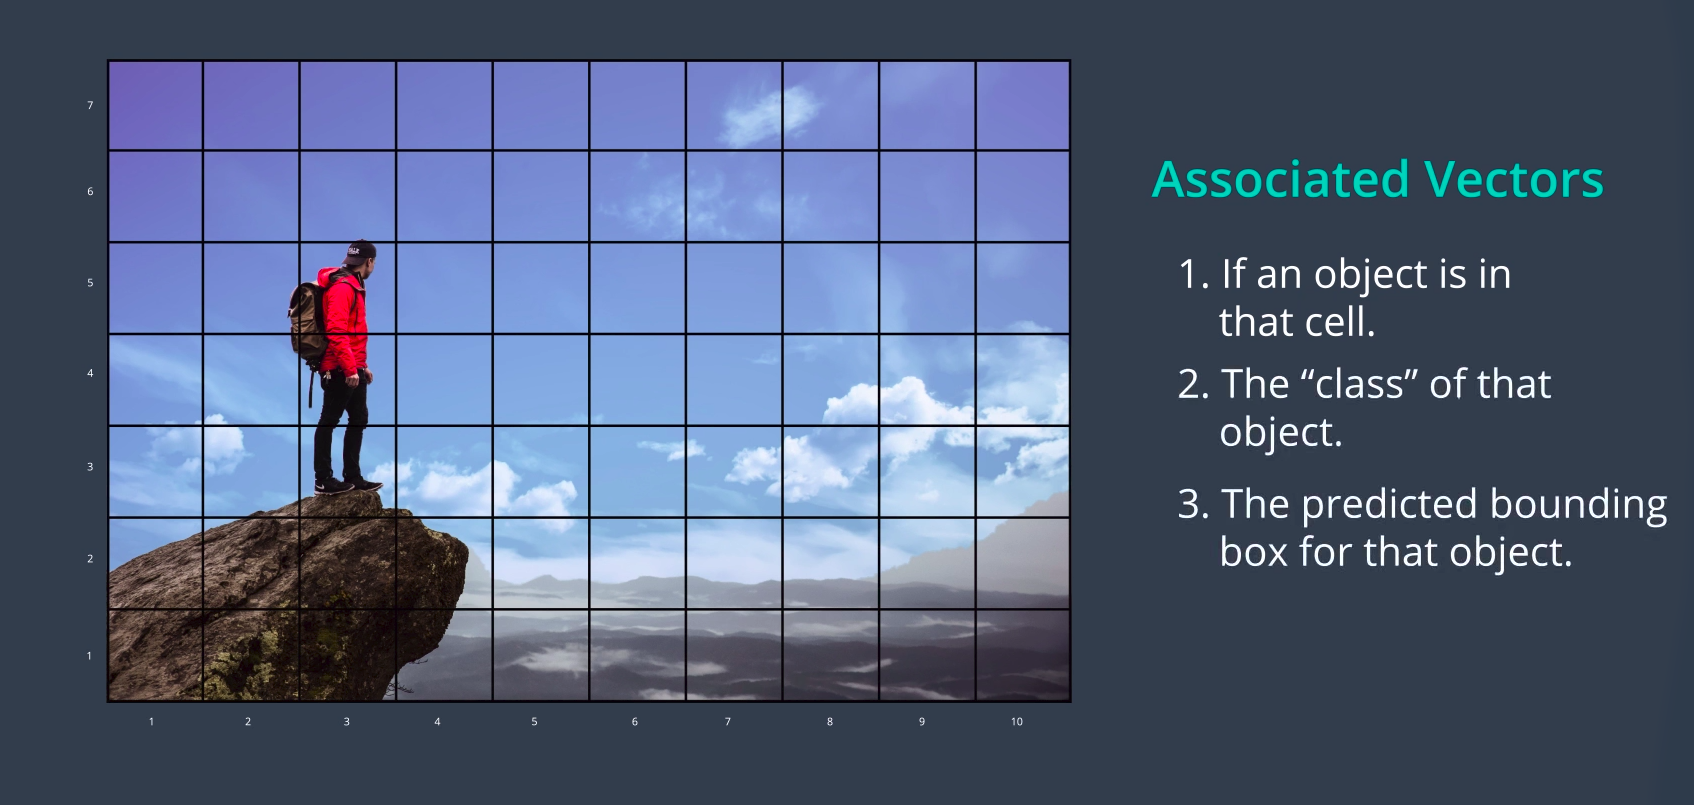
\includegraphics[height=0.7\textheight]{grid}
\end{frame}
}


{\usebackgroundtemplate{
\includegraphics[width=1.0\paperwidth]{background}}%
\begin{frame}
\frametitle{A grid instead windows}
\framesubtitle{Improving localization}
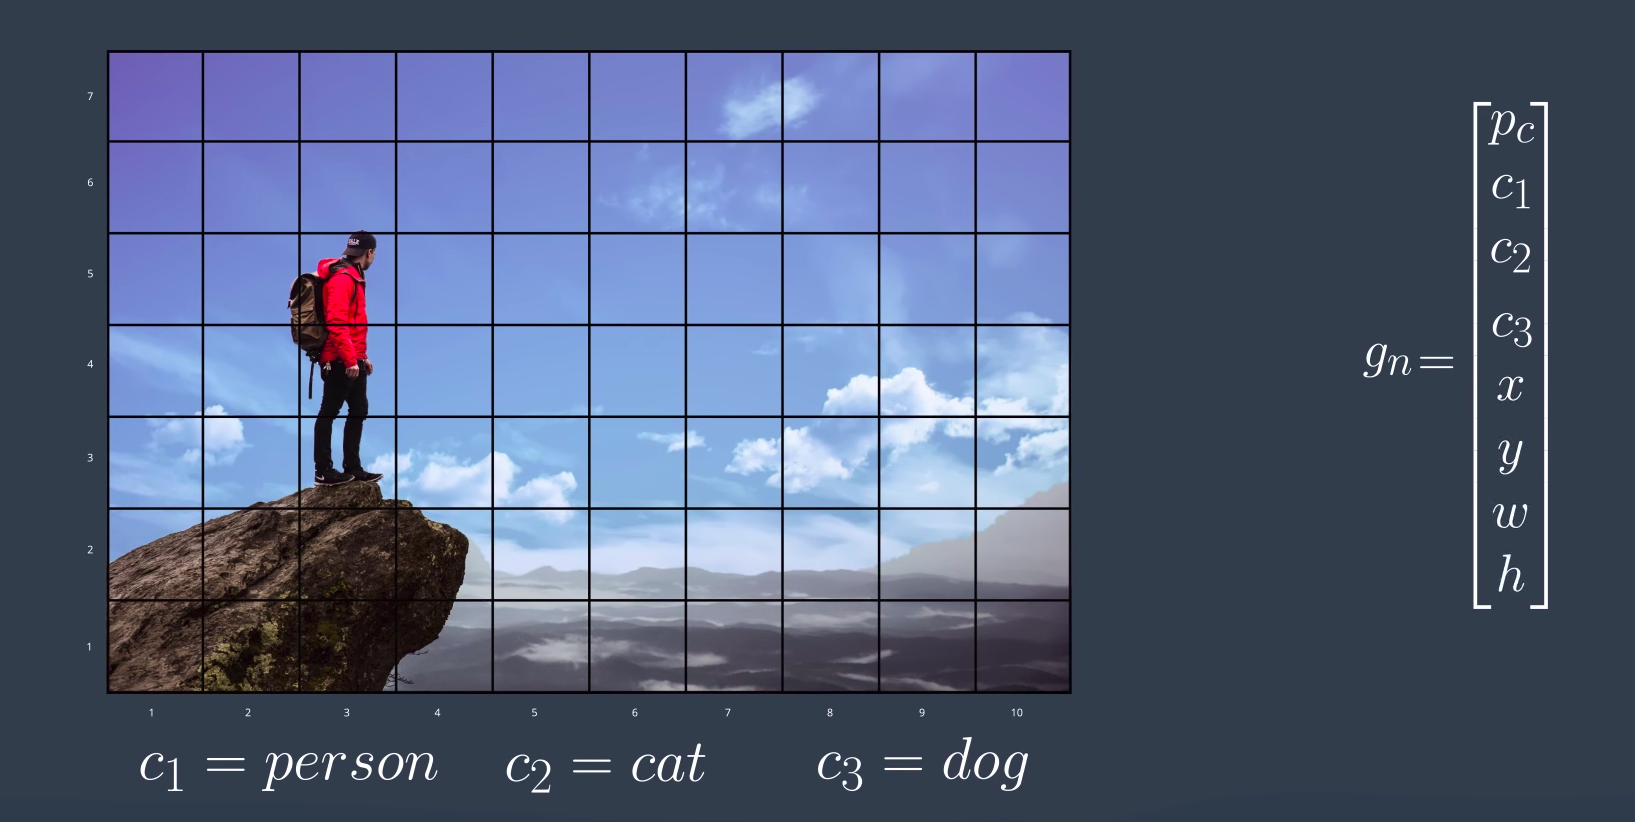
\includegraphics[height=0.7\textheight]{grid2}
\end{frame}
}


{\usebackgroundtemplate{
\includegraphics[width=1.0\paperwidth]{background}}%
\begin{frame}
\frametitle{Training labels}
\begin{figure}
	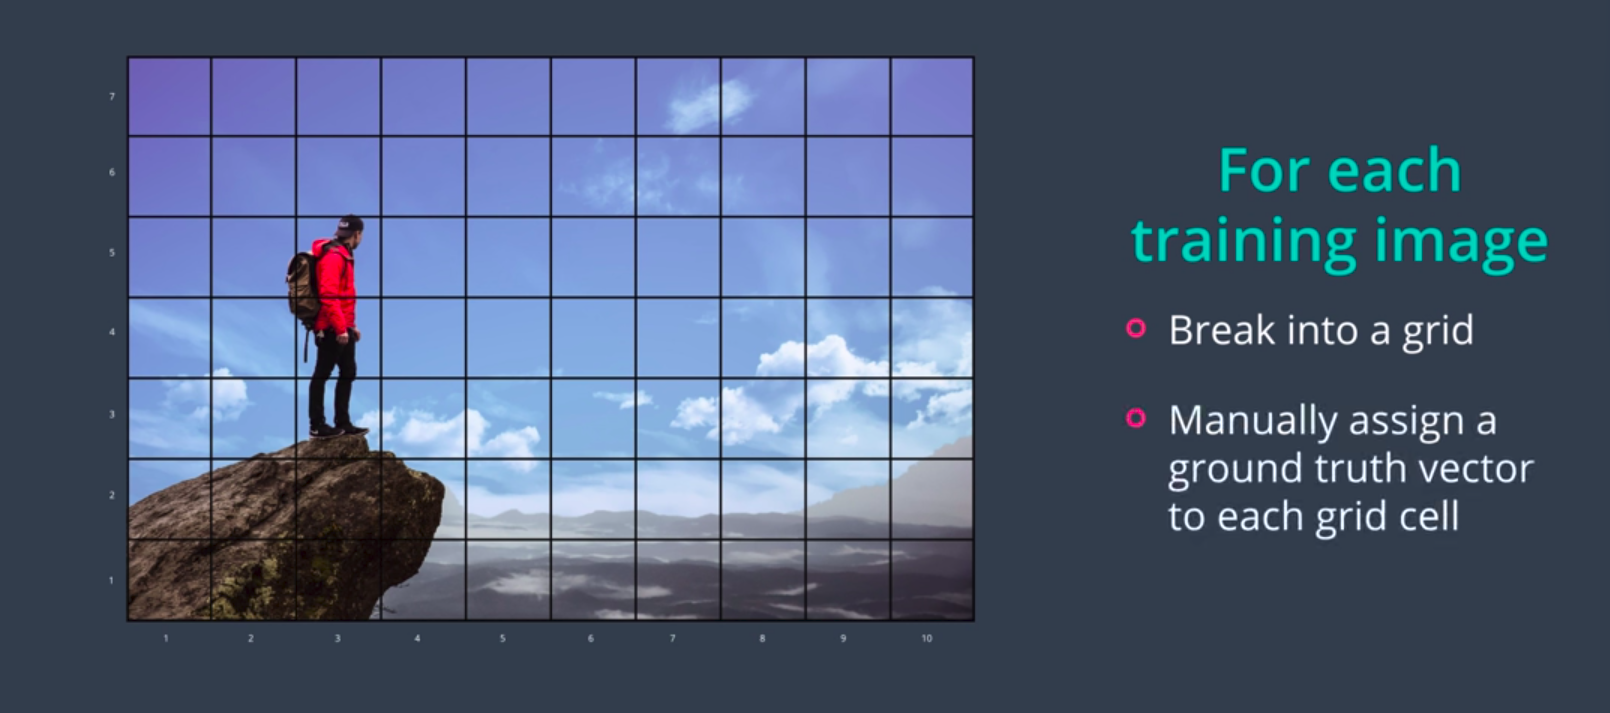
\includegraphics[height=0.6\textheight]{train1}
\end{figure}
\end{frame}
}


{\usebackgroundtemplate{
\includegraphics[width=1.0\paperwidth]{background}}%
\begin{frame}
\frametitle{Training labels}
\begin{figure}
	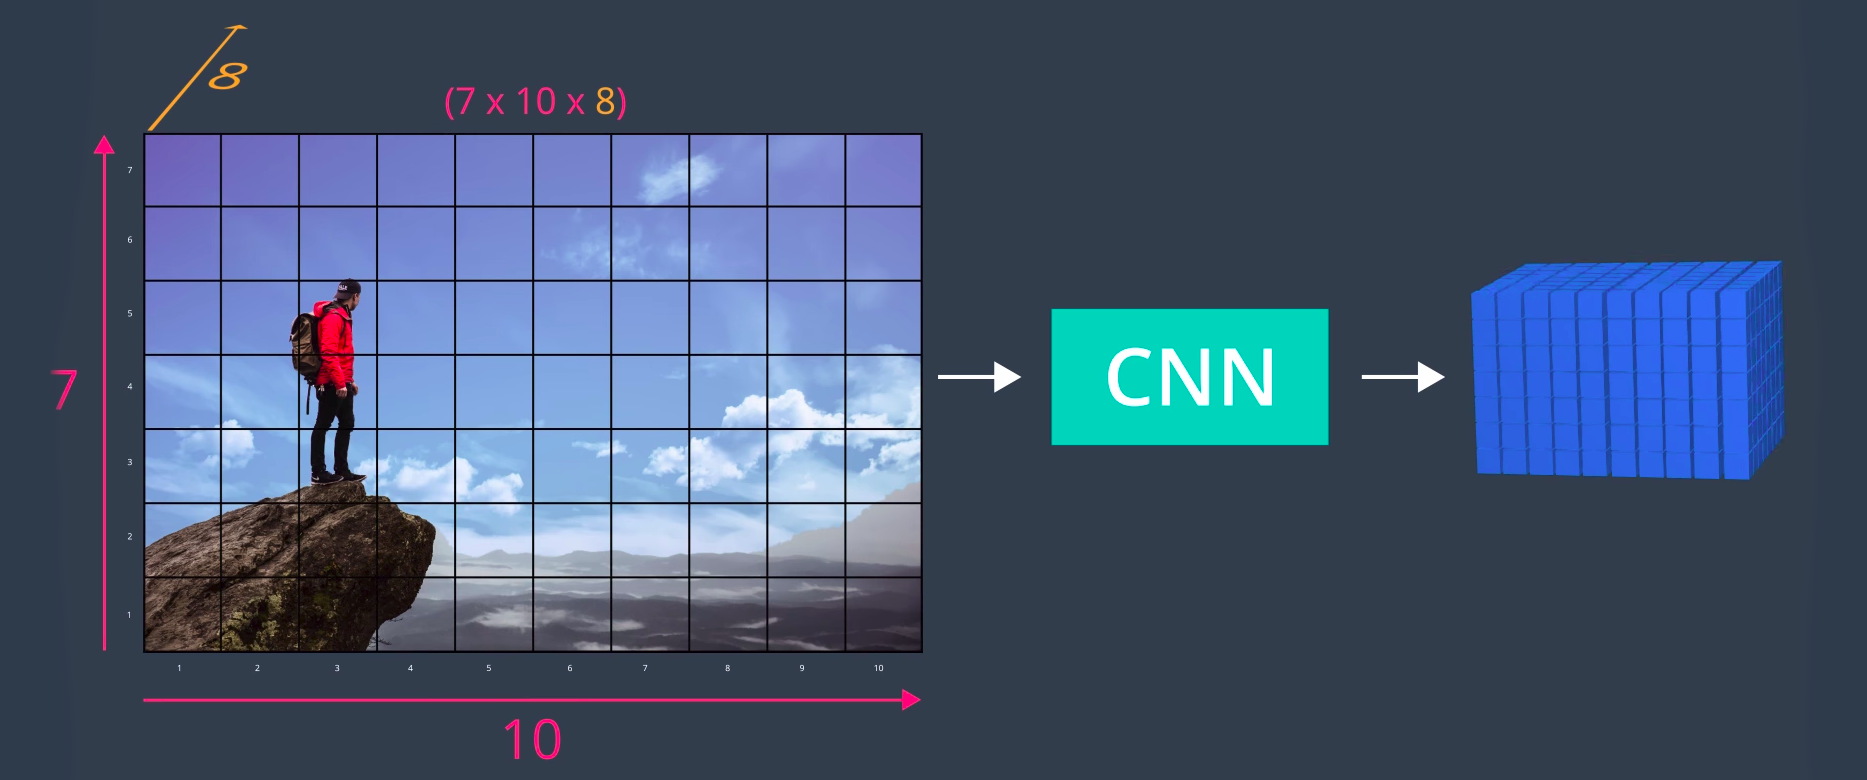
\includegraphics[height=0.6\textheight]{train2}
\end{figure}
\end{frame}
}


{\usebackgroundtemplate{
\includegraphics[width=1.0\paperwidth]{background}}%
\begin{frame}
\frametitle{Training labels}
\begin{figure}
	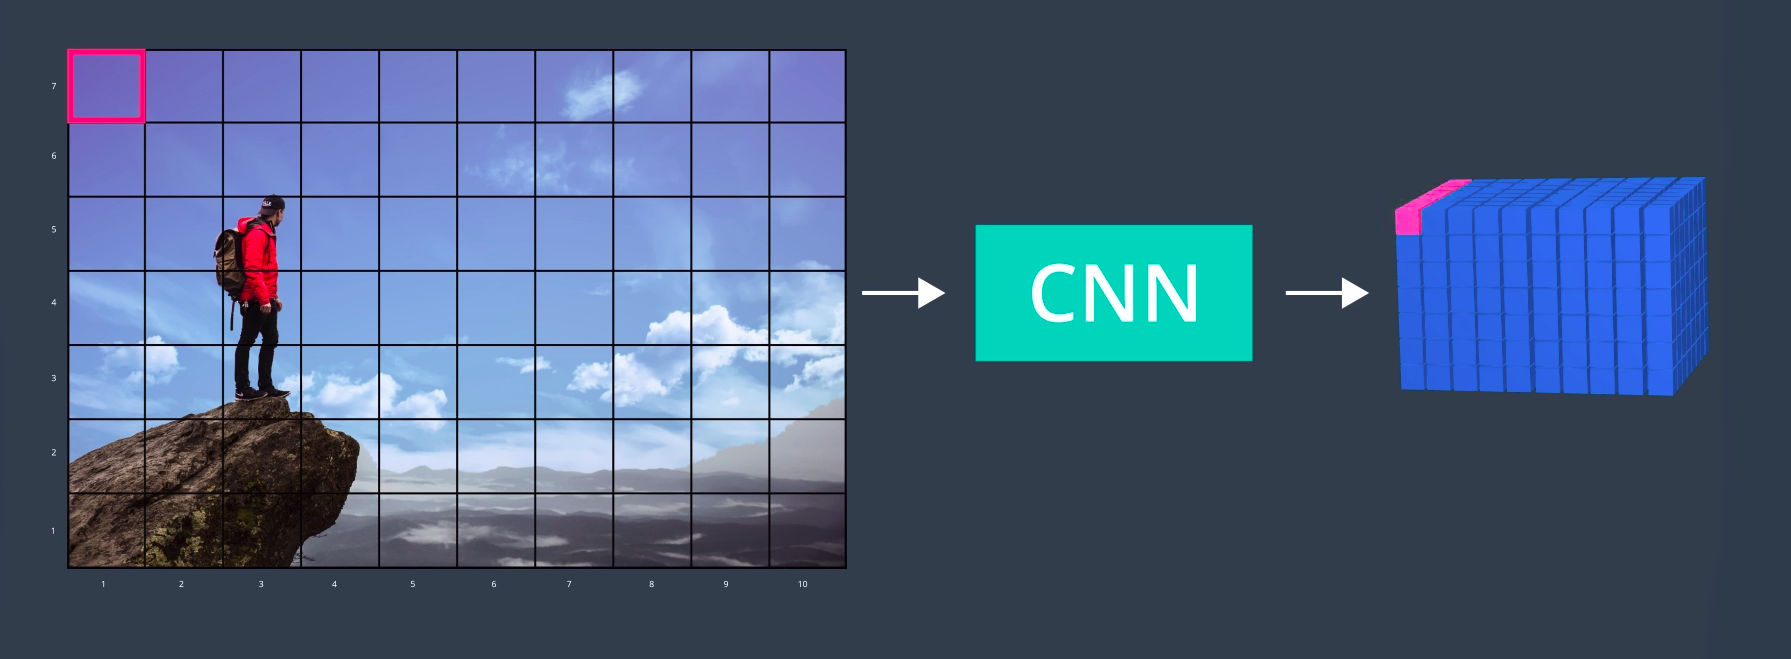
\includegraphics[height=0.6\textheight]{train3}
\end{figure}
\end{frame}
}


{\usebackgroundtemplate{
\includegraphics[width=1.0\paperwidth]{background}}%
\begin{frame}
\frametitle{Training labels}
\begin{itemize}
	\item \textcolor{white}{Training locations.}
	\item \textcolor{white}{The location of one object is assign to only one grid cell.}
\end{itemize}
\begin{figure}
	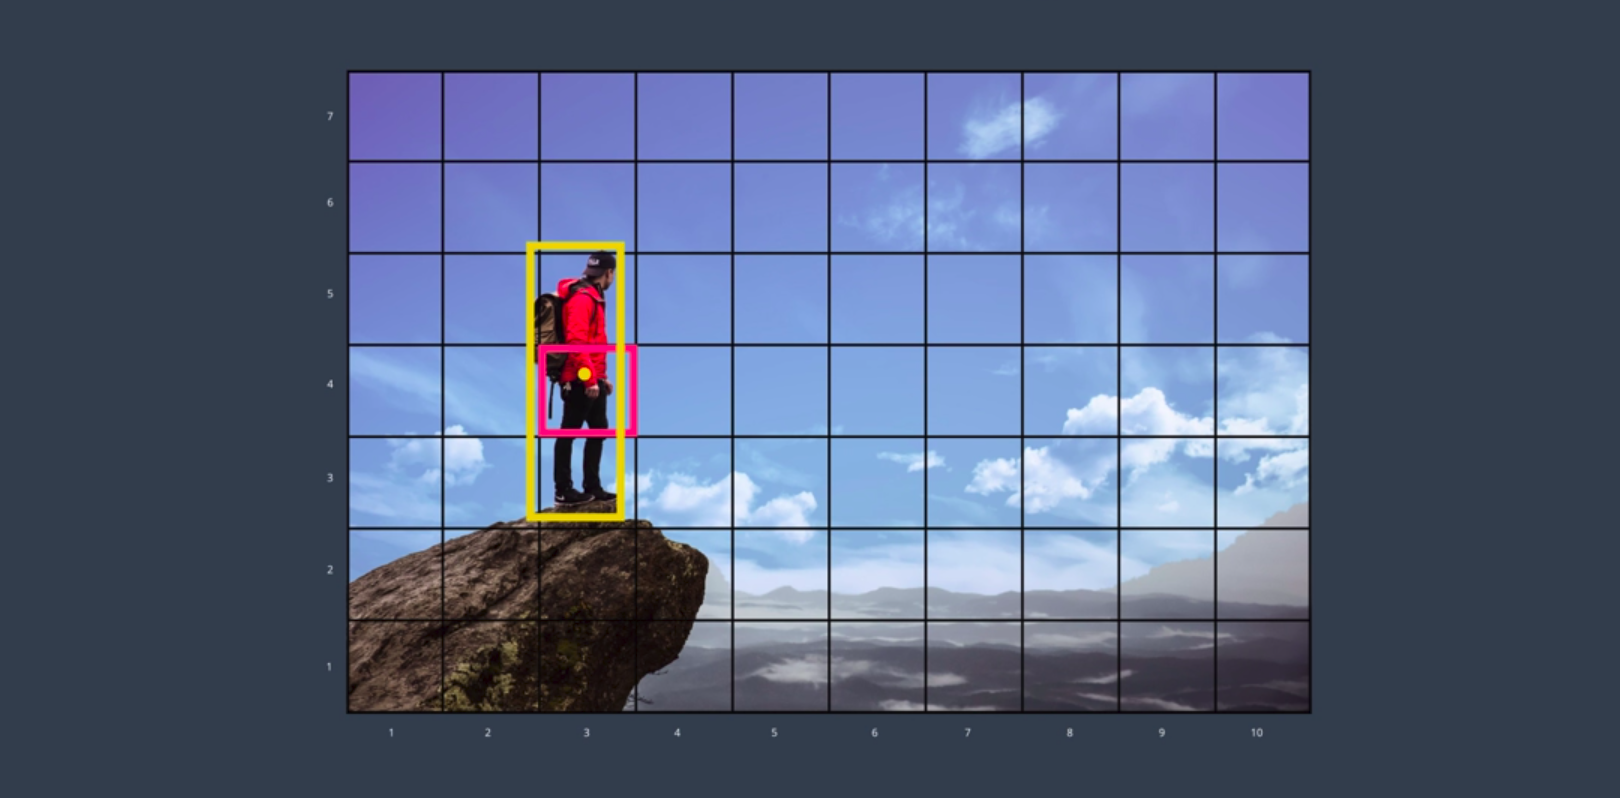
\includegraphics[height=0.6\textheight]{pos1}
\end{figure}
\end{frame}
}


{\usebackgroundtemplate{
\includegraphics[width=1.0\paperwidth]{background}}
\begin{frame}
\frametitle{Training labels}
\begin{itemize}
	\item \textcolor{white}{The center of the object is relative to the cell.}
\end{itemize}
%\begin{figure}
	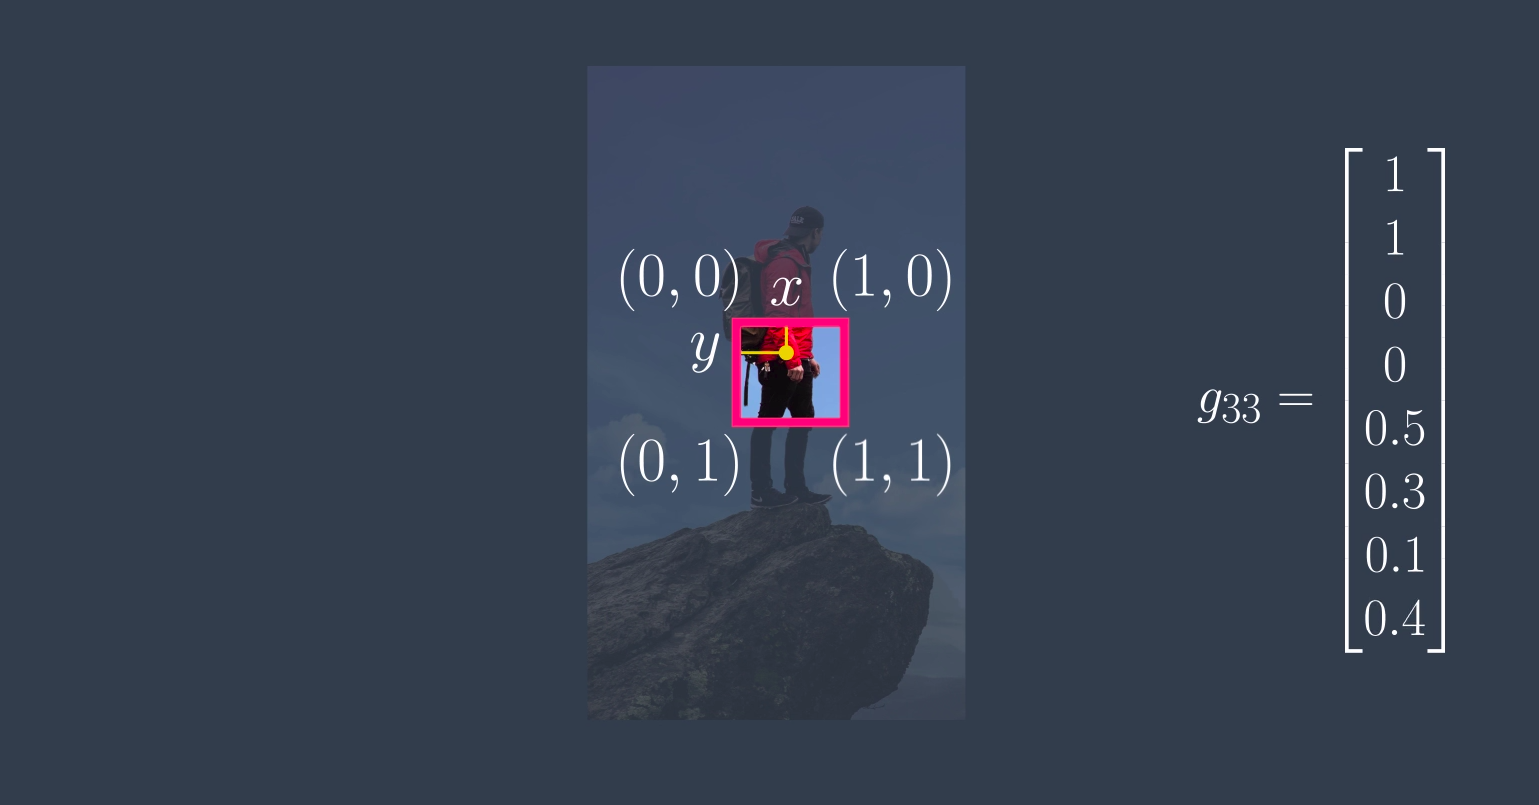
\includegraphics[height=0.7\textheight]{pos2}
%\end{figure}
\end{frame}
}


{\usebackgroundtemplate{
\includegraphics[width=1.0\paperwidth]{background}}
\begin{frame}
\frametitle{Training labels}
\begin{itemize}
	\item \textcolor{white}{The width and height are relative to the image.}
\end{itemize}
\begin{figure}
	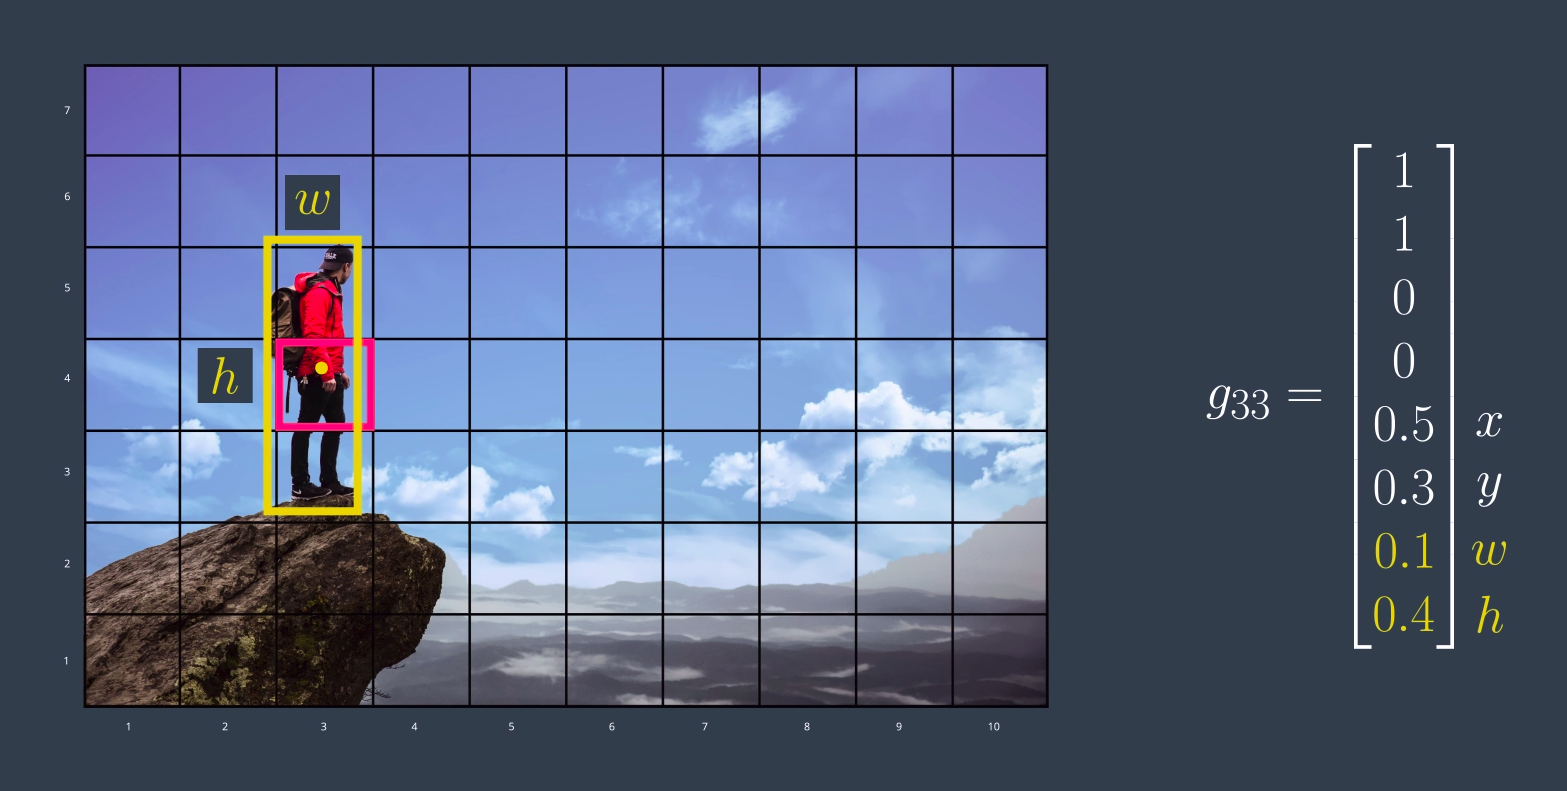
\includegraphics[height=0.6\textheight]{pos3}
\end{figure}

\end{frame}
}


\begin{frame}
\frametitle{Quiz}
\begin{itemize}
	\item Wich cell will provide the correct label?
\end{itemize}
\begin{figure}
	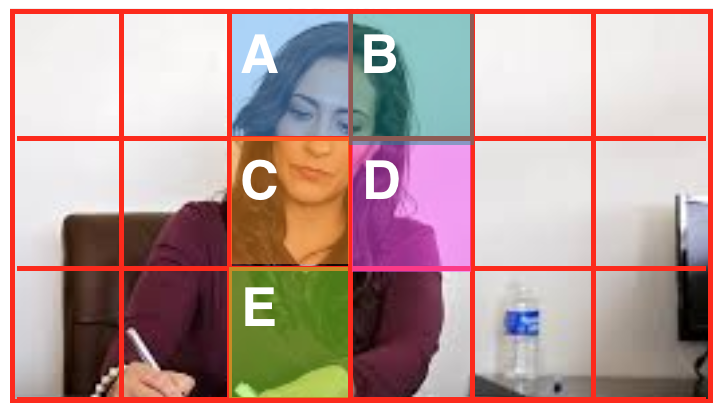
\includegraphics[height=0.6\textheight]{test1}
\end{figure}
\end{frame}


{\usebackgroundtemplate{
\includegraphics[width=1.0\paperwidth]{background}}
\begin{frame}
\frametitle{Multiple boxes}
\begin{itemize}
	\item \textcolor{white}{A problem with grid cells is that they provide too many boxes.}
\end{itemize}
\begin{figure}
	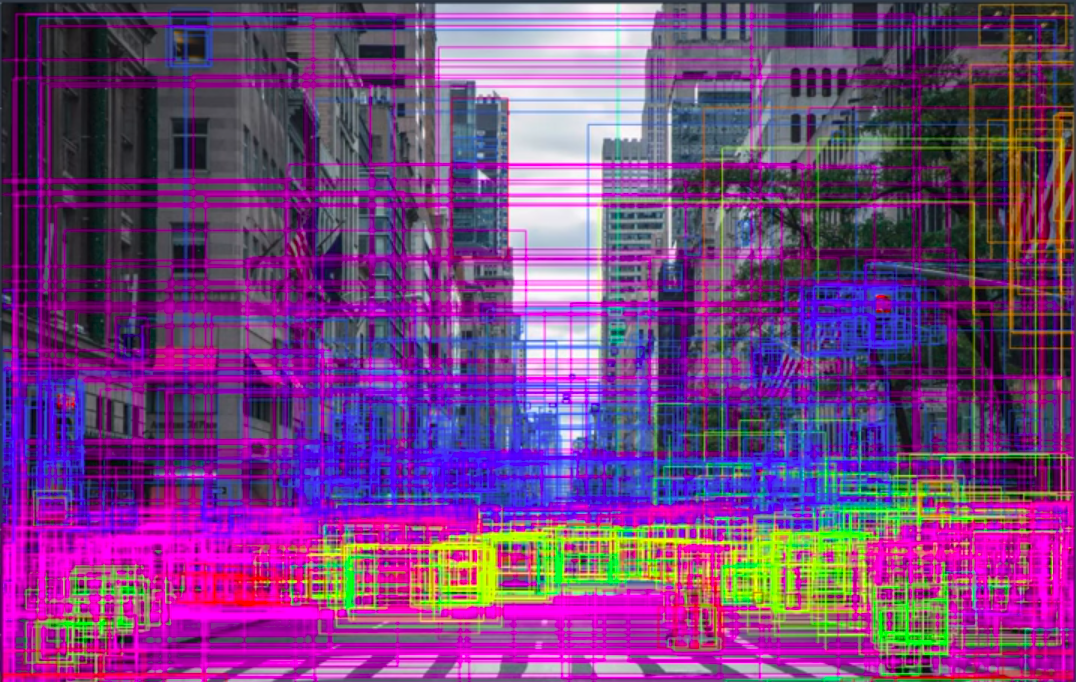
\includegraphics[height=0.7\textheight]{boxes}
\end{figure}
\end{frame}
}


\begin{frame}
\frametitle{Non Maximum suppression}
\begin{itemize}
	\item Intersection over union
		\begin{equation}
			IOU = \dfrac{A_{intersection}}{A_{union}}
		\end{equation}
		\begin{center}
			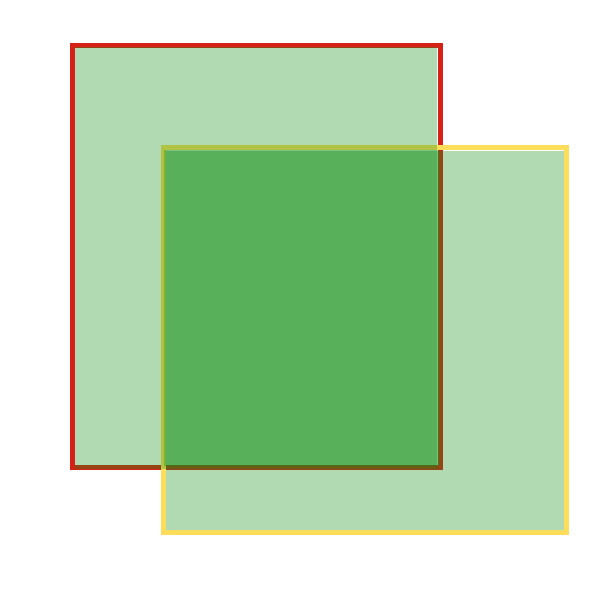
\includegraphics[height=0.5\textheight]{iou}
		\end{center}
	\item What is the range of the function?
\end{itemize}
\end{frame}


\begin{frame}
\frametitle{Non Maximum suppression}
\begin{enumerate}
	\item Look at the output vector of each grid cell. 
	\item Remove all bounding boxes that have a $p_c$ value less than or equal to some threshold. $$ p_c < 0.5$$ 
	\item Select the bounding box with the highest $p_c$ value.
	\item Remove all the bounding boxes that have a high $IoU$ with the box selected in the last step.
\end{enumerate}
\end{frame}


{\usebackgroundtemplate{
\includegraphics[width=1.0\paperwidth]{background}}
\begin{frame}
\frametitle{Anchor boxes}
\begin{itemize}
	\item \textcolor{white}{Same center problem.}
\end{itemize}
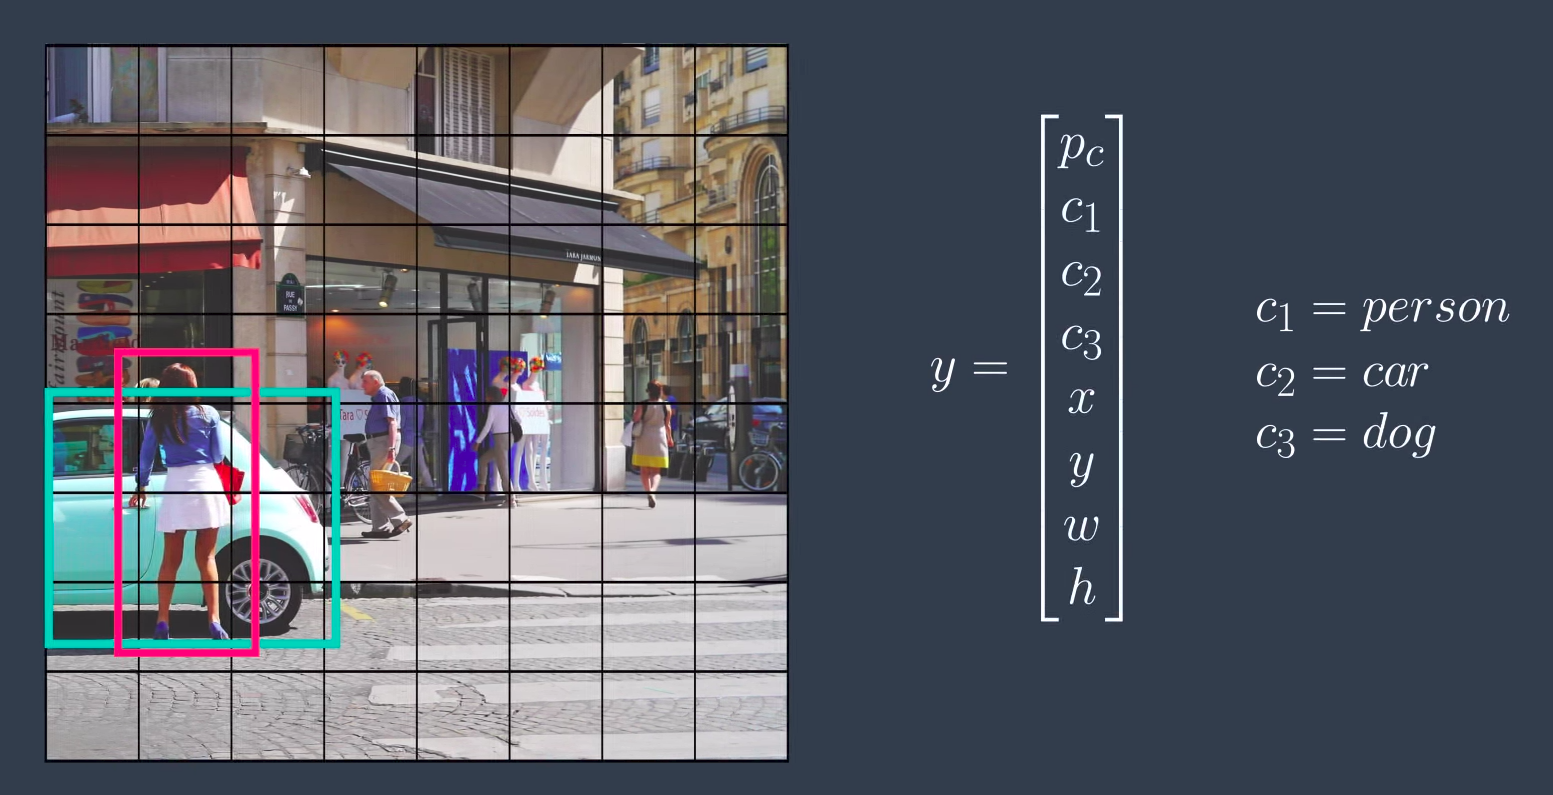
\includegraphics[height=0.7\textheight]{anchor1}
\end{frame}
}


{\usebackgroundtemplate{
\includegraphics[width=1.0\paperwidth]{background}}
\begin{frame}
\frametitle{Anchor boxes}
\begin{itemize}
	\item \textcolor{white}{Each anchor box as different aspect ratio.}
\end{itemize}
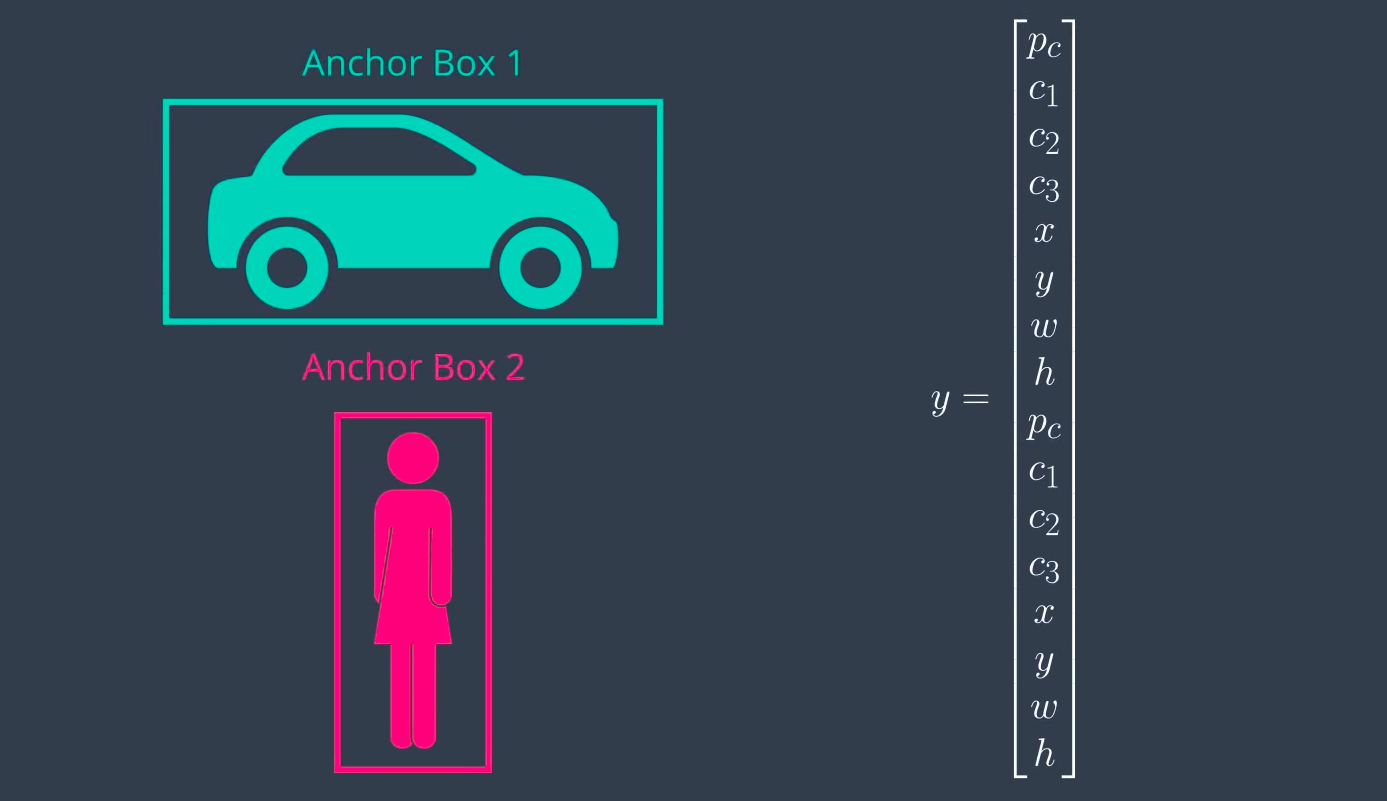
\includegraphics[height=0.7\textheight]{anchor2}
\end{frame}
}


{\usebackgroundtemplate{
\includegraphics[width=1.0\paperwidth]{background}}
\begin{frame}
\frametitle{Anchor boxes}
\begin{itemize}
	\item \textcolor{white}{We can place as many anchor boxes as we want.}
\end{itemize}
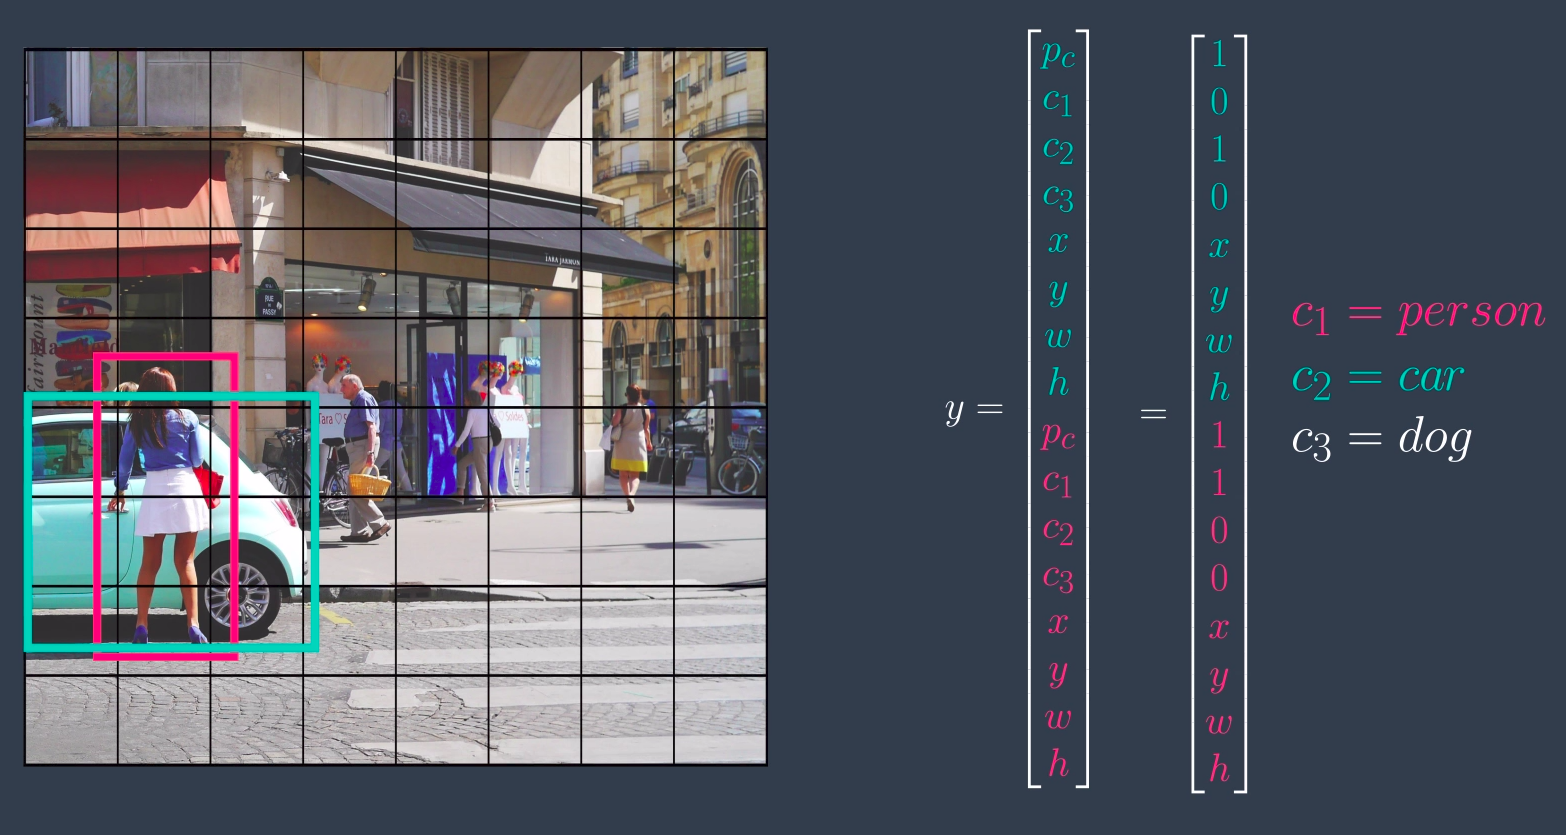
\includegraphics[height=0.7\textheight]{anchor3}
\end{frame}
}


\begin{frame}
\frametitle{YOLO Architecture}
%\begin{itemize}
%\item Done
%\end{itemize}
\begin{figure}
	\centering
	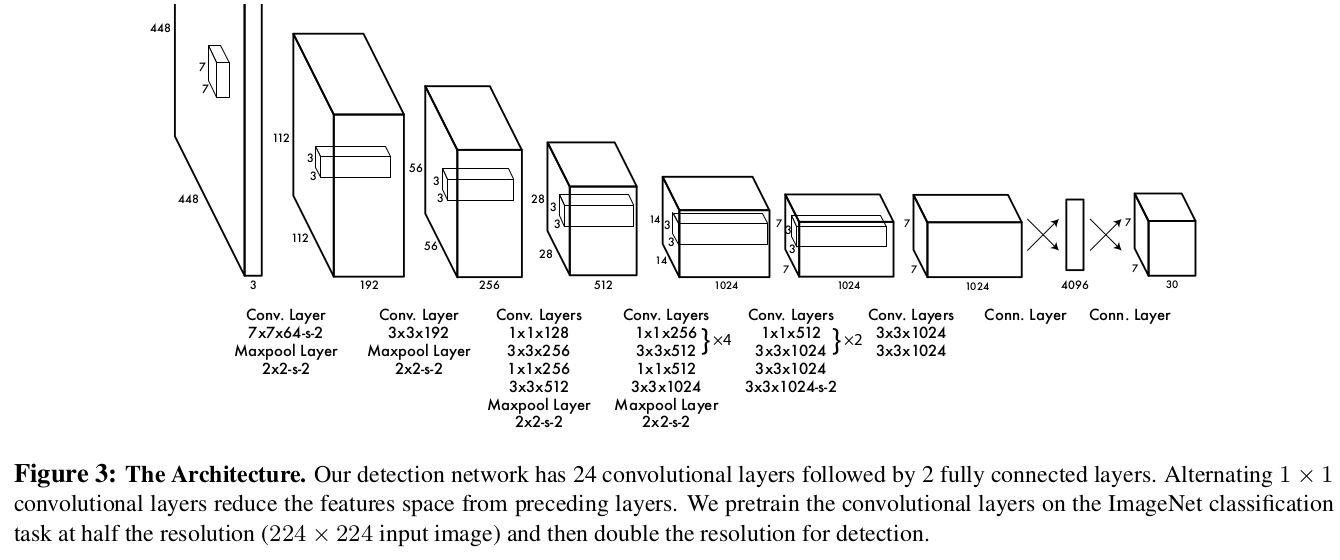
\includegraphics[height=0.7\textheight]{yoloarchitecture}
	%\caption{}
	\label{fig:yoloarchitecture}
\end{figure}
\end{frame}



\begin{frame}
	\frametitle{YOLO Results}
%	\begin{itemize}
%		\item Done
%	\end{itemize}
\begin{figure}
	\centering
	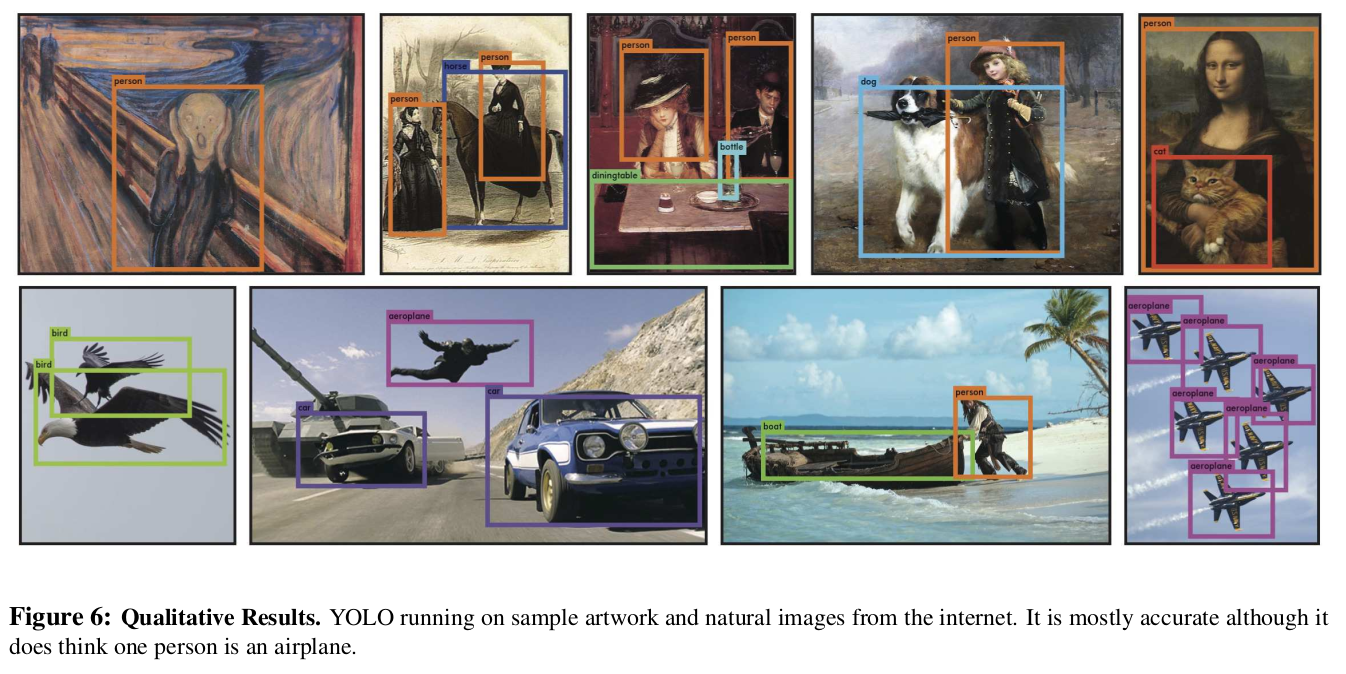
\includegraphics[height=0.7\textheight]{yoloresults}
	%\caption{}
	\label{fig:yoloresults}
\end{figure}
\end{frame}




\begin{frame}
\frametitle{References}
\begin{itemize}
	\item Redmon, Joseph, et al. "You only look once: Unified, real-time object detection." Proceedings of the IEEE conference on computer vision and pattern recognition. 2016.
	\item Goodfellow, I., Bengio, Y., Courville, A., \& Bengio, Y. (2016). Deep learning (Vol. 1). Cambridge: MIT press.
	\item Alex Smola and S.V.N. Vishwanathan, Introduction to Machine Learning, Cambirdge University Press.
	\item Udacity, Computer vision nanodegree
\end{itemize}
\end{frame}

\end{document}